\newpage

\chapter{Apêndice 2}
\label{apendice2}

\section{Descrição de testes de aceitação}

Essa estrutura é proposta da seguinte forma:

\begin{enumerate}
\item \textbf{Título:} Palavra-chave ‘\textit{feature}’ e um título curto que representa o 
objetivo da \textit{feature}.
\item \textbf{Narrativa:} um texto curto que demonstre os cenários de execução, 
exatamente como a narrativa de uma história de usuário:

\begin{figure}[!h]
    \centering
    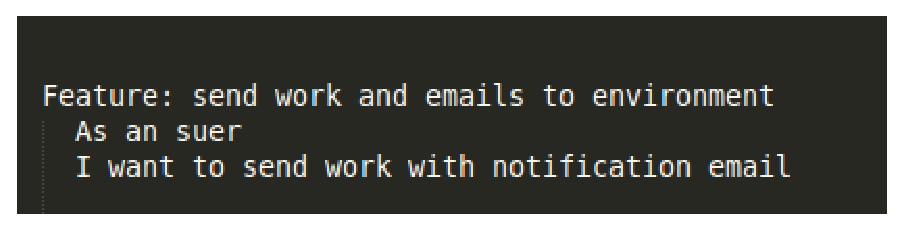
\includegraphics[keepaspectratio=true,scale=0.50]
      {figuras/noosfero_feature2.eps}
    \caption{Descrição do título (\textit{feature}) de um teste}
    \label{nosfero_feature}
\end{figure}

\item \textbf{Pré condições:} representado pela palavra-chave \textit{'background'}, define os passos 
precedem cada cenário de teste.

\begin{figure}[!h]
    \centering
    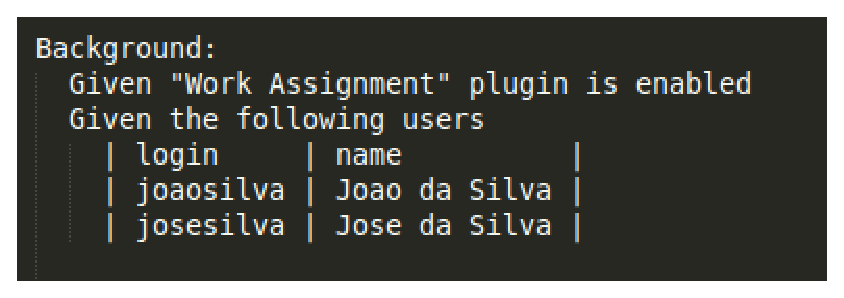
\includegraphics[keepaspectratio=true,scale=0.50]
      {figuras/noosfero_back.eps}
    \caption{Descrição de pré condições (\textit{background}) de um teste}
    \label{nosfero_feature}
\end{figure}

\item \textbf{Cenários:} representam parte concreta de como o software deve se 
comportar, e sendo a parte essencial do teste realizado no 
cucumber. Após a palavra-chave \textit{‘scenario’} define-se o nome do cenário em questão:
\item \textbf{Passos:} Cada cenário possui uma série de passos que demonstram o seu 
comportamento, que são linhas simples iniciadas com as seguintes palavras-chaves: 
\textit{Given, When, Then, And, But}.
\item \textbf{Given:} Indica uma condição inicial para que o cenário seja executado, 
trata-se das pré-condições do cenário.
\item \textbf{When:} Indica o evento do cenário
\item \textbf{Then:} Indica o que é esperado após o evento ocorrer.

\begin{figure}[!h]
    \centering
    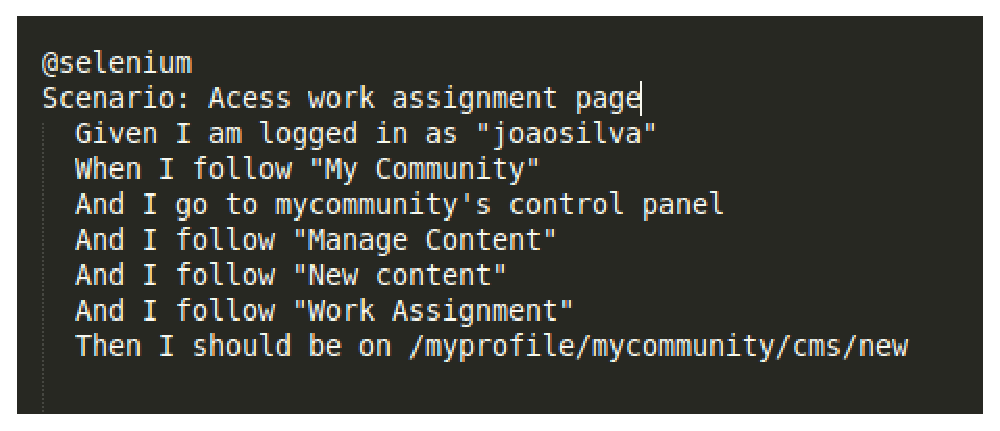
\includegraphics[keepaspectratio=true,scale=0.50]
      {figuras/noosfero_scenario.eps}
    \caption{Descrição do cenário (\textit{scenario}) de um teste}
    \label{nosfero_scenario}
\end{figure}

\end{enumerate}

\section {Descrição de funcionais e unitários}

Os testes funcionais e unitários são escritos da seguinte forma:

\textbf{Setup:} indica as condições inciais dos testes, setando variáveis de ambiente e de configuração por exemplo.

\begin{figure}[!h]
    \centering
    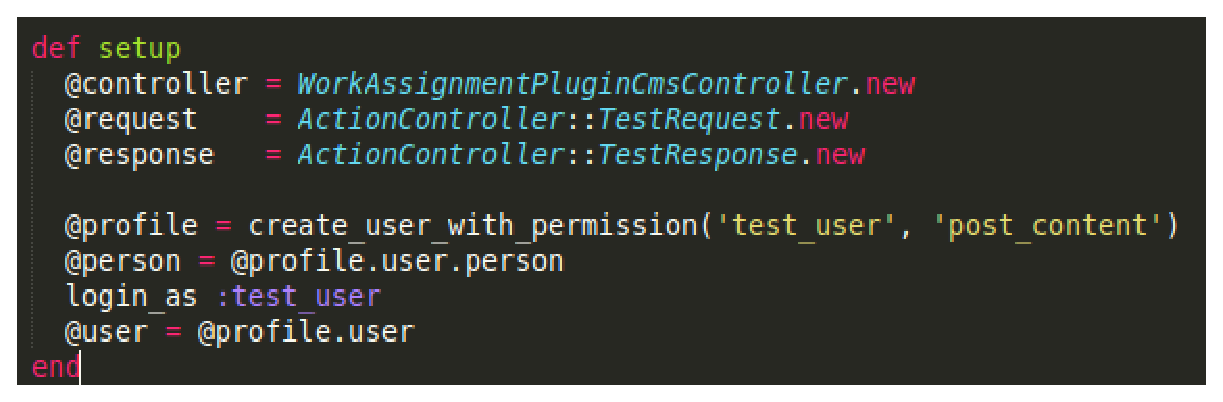
\includegraphics[keepaspectratio=true,scale=0.5]
      {figuras/teste_setup.eps}
    \caption{Descrição do setup de um teste}
    \label{nosfero_setup}
\end{figure}

\textbf{Título:} título do teste iniciado com a palavra \textit{‘should’} e finalizado com \textit{‘do’}

\textbf{Passos:} código que define o comportamento do teste

\textbf{Verificação:} Assertiva que verifica se a ação foi realizada como esperada.

\begin{figure}[!h]
    \centering
    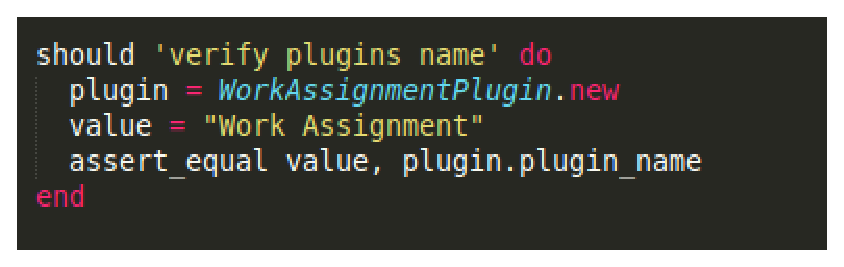
\includegraphics[keepaspectratio=true,scale=0.55]
      {figuras/teste_should.eps}
    \caption{Código de teste}
    \label{noosfero_should}
\end{figure}

\section{Cenários de Uso da release 0}
\label{cenario_uso}
    Os cenários de uso foram a base de criação dos testes de aceitação.
    Durante a primeira release (release 0) foram desenvolvidas algumas histórias, dentre estas, a história de ``Cadastro de Usuário'', que possui os seguintes cenários de sucesso:

    \begin{itemize}
    \item\textbf{Cenário 01:} Cadastro com sucesso de apenas campos obrigatórios

    \textbf{[Dado]} que não existe nenhum usuário com o nome de usuário ``josesilva''

    \textbf{[Quando]} eu clicar em cadastrar novo usuário

    \textbf{[E]} eu preencho os seguintes campos: 

        \subitem nome de usuário: ``josesilva''

        \subitem e-mail: ``jose@gmail.com''

        \subitem senha: ``123456''

        \subitem confirmação da senha: ``123456''

        \subitem nome completo: ``José da Silva''

        \subitem país: ``Brasil''

        \subitem estado: ``Distrito Federal''

        \subitem cidade: ``Brasília''

    \textbf{[E]} eu clico em cadastrar

    \textbf{[Então]} eu recebo uma confirmação de cadastro realizado com sucesso


    \item\textbf{Cenário 02:} Cadastro com sucesso de apenas campos obrigatórios de usuário governamental
    
    \textbf{[Dado]} que não existe nenhum usuário com o nome de usuário ``josesilva''
    
    \textbf{[Quando]} eu clicar em cadastrar novo usuário
    
    \textbf{[E]} eu preencho os seguintes campos: 
        \subitem nome de usuário: ``josesilva''

        \subitem e-mail: ``jose@serpro.gov.br''

        \subitem e-mail secundário: ``jose@gmail.com''

        \subitem senha: ``123456''

        \subitem confirmação da senha: ``123456''

        \subitem nome completo: ``José da Silva''

        \subitem cargo: ``analista de TI''

        \subitem país: ``Brasil''

         \subitem estado: ``Distrito Federal''

        \subitem cidade: ``Brasília''

    \textbf{[E]} eu seleciono ``SERPRO'' como instituição

    \textbf{[E]} eu seleciono ``teste'' como unidade  

    \textbf{[E]} eu clico em cadastrar

    \textbf{[Então]}eu recebo uma confirmação de cadastro realizado com sucesso

\item\textbf{Cenário 3:} Cadastro com sucesso com todos os campos preenchidos, mesmo não obrigatórios

    \textbf{[Dado]} que não existe um usuário cujo email primário ou email secundário é ``maria@gmail.com''

    \textbf{[Quando]} eu clicar em cadastrar novo usuário

    \textbf{[E]} eu preencho os seguintes campos: 

        \subitem nome de usuário: ``mariasilva''

          \subitem e-mail: ``maria@gmail.com''

          \subitem e-mail secundário: ``maria@yahoo.com''

          \subitem senha: ``123456''

          \subitem confirmação da senha: ``123456''

          \subitem nome completo: ``Maria da Silva''

          \subitem cargo: ``analista de TI''

          \subitem áreas de interesse: ``Engenharia de Software''

          \subitem país: ``Brasil''

          \subitem estado: ``Distrito Federal''

          \subitem cidade: ``Brasília''

    \textbf{[E]} eu seleciono ``Outro'' como instituição 

    \textbf{[E]} eu clico em cadastrar

    \textbf{[Então]} eu recebo uma notificação de cadastro realizado com sucesso.
    \end{itemize}

    Os cenários de falha ocorrem nas seguintes situações:
    \begin{itemize}
    \item Email proposto existir como email de outro usuário;
    \item Email secundário proposto existir como email de outro usuário;
    \item Email secundário ser um email governamental e ao email primário não ser um email governamental;
    \item Não preenchimento de campos obrigatórios para usuário governamental 
    \end{itemize}

     Quanto a história chamada ``Manter Instituição''  possui os seguintes cenários:

\begin{itemize}
\item\textbf{Cenário 01:} Cadastro de nova instituição com sucesso

\textbf{[Dado]} que eu estou na página de cadastro de usuário

\textbf{[E]} que a seguinte instituição não existe:

    \subitem nome: ``Ministério do Planejamento, Orçamento e Gestão''

    \subitem sigla: ``MP''

    \subitem poder: ``executivo''

    \subitem esfera: ``federal''

    \subitem tipo: ``pública''

    \subitem cnpj: ``00.489.828/0002-36''

\textbf{[Quando]} eu clicar em ``Cadastrar nova instituição''

\textbf{[E]} eu preencher os seguintes campos:

    \subitem sigla: ``MP''

    \subitem poder: ``executivo''

    \subitem esfera: ``federal''

    \subitem tipo: ``pública''

    \subitem cnpj: ``00.489.828/0002-36''

\textbf{[Então]} eu devo visualizar a mensagem ``Instituição cadastrada com sucesso!''

\item\textbf{Cenário 02:} Busca de instituição inexistente

\textbf{[Dado]} que eu estou na página de cadastro de usuário

\textbf{[E]} que a seguinte instituição não existe:

 \subitem nome: ``Ministério do Planejamento, Orçamento e Gestão''

  \subitem sigla: ``MP''

  \subitem poder: ``executivo''

  \subitem esfera: ``federal''

  \subitem tipo: ``pública''
  
  \subitem cnpj: ``00.489.828/0002-36''

\textbf{[Quando]} eu buscar MP

\textbf{[Então]} eu devo visualizar a mensagem ``Instituição não cadastrada''

\textbf{[E]}eu devo visualizar a opção de cadastrar nova instituição
\end{itemize}

\section{Cenários de Uso da release 1}
\label{cenario_r1}


Durante a segunda release (release 1) a história de ``Cadastro de Usuário'' foi desenvolvida novamente com o seguinte cenário:

\begin{itemize}
\item\textbf{Cenário 01:} Cadastro com sucesso de apenas campos obrigatórios

    \textbf{[Dado]} que não existe nenhum usuário com o nome de usuário ``josesilva''

    \textbf{[Quando]} eu clicar em ``Cadastre-se''

    \textbf{[E]} eu preencho os seguintes campos: 

        \subitem primeiro nome: ``José''

        \subitem ultimo nome: ``Silva''

        \subitem endereço de e-mail: ``jose@gmail.com''

        \subitem usuário: ``josesilva''
        
    \textbf{[E]} eu clico em ``Cadastre-se''

    \textbf{[Então]} eu recebo uma confirmação de cadastro realizado com sucesso, com a seguinte mensagem: 
    ``Você deve se logar para seu perfil. Perfis não validados serão deletados em 24h.''
\end{itemize}

\section{Cenários de uso da release 2}
\label{cenario_r2}

Durante a segunda release (release 2) a história de ``Novo Software'' foi desenvolvida com os seguintes cenários:

\begin{itemize}
\item\textbf{Cenário 01:} Novo Software

    \textbf{[Dado]} que não existe nenhum software com o localhost ``software''

    \textbf{[Quando]} eu clicar em ``Novo Software''

    \textbf{[E]} eu preencho os seguintes campos: 

        \subitem localhost: ``software''

        \subitem finalidade: ``Finalidade do software''

        \subitem licenca: ``licença''
        
        
    \textbf{[E]} eu clico em ``Salvar''

    \textbf{[Então]} eu recebo uma confirmação de cadastro realizado com sucesso, e encontro a pagina de edição de software


Outros cenários de edição de software são: ``Informações de Comunidade'' e ``Informações de Software''.

\item\textbf{Cenário 02:} Informações de Comunidade

    \textbf{[Dado]} que ``software'' está cadastrado

    \textbf{[Quando]} eu clicar em ``Cadastre-se''

    \textbf{[E]} eu preencho os seguintes campos: 

        \subitem descricao: ``Descrição do software''

        \subitem tags: ``software''

        \subitem categorias: ``categoria1''
 
    \textbf{[E]} eu clico em ``Salvar''

    \textbf{[Então]} eu recebo uma confirmação de cadastro salvo com sucesso


\item\textbf{Cenário 03:} Informações de Software

    \textbf{[Dado]} que ``software'' está cadastrado e estou em Edição de software

    \textbf{[Quando]} eu clicar em ``Especifico''

    \textbf{[E]} eu preencho os seguintes campos: 

        \subitem Sigla: ``teste''

        \subitem sistema operacional: ``teste os''

        \subitem funcionalidades: ``testes''

        \subitem categorias: ``categoria1''
    
    \textbf{[E]} eu clico em ``Nova Biblioteca''

    \textbf{[E]} eu preencho os seguintes campos: 

        \subitem nome: ``teste''

        \subitem versão: ``teste''

        \subitem licença: ``teste''

    \textbf{[E]} eu clico em ``Novo Sistema Operacional''

    \textbf{[E]} eu preencho os seguintes campos: 

        \subitem nome: ``Debian''

        \subitem versão: ``teste''

    \textbf{[E]} eu clico em ``Nova linguagem''

    \textbf{[E]} eu preencho os seguintes campos: 

        \subitem nome: ``C++''

        \subitem versão: ``teste''

        \subitem sistema operacional: ``Debian''

    \textbf{[E]} eu clico em ``Novo Banco de Dados''

    \textbf{[E]} eu preencho os seguintes campos: 

        \subitem nome: ``apache''

        \subitem versão: ``teste''

        \subitem sistema operacional: ``Debian''

    \textbf{[E]} eu clico em ``Salvar''

    \textbf{[Então]} eu recebo uma confirmação de cadastro salvo com sucesso
    
    
\end{itemize}

\newpage

\section{Pesquisa com profissionais de software livre e métodos ágeis}

	Foi realizada uma pesquisa para entender o que profissionais que trabalham com software livre e métodos ágeis entendem sobre as técnicas de usabilidade. O resultado se encontram abaixo:
	
	A grande maioria dos profissionais pesquisados eram desenvolvedores, seguidos de designs, arquitetos de informação, especialistas de usabilidade e gerentes de projetos. Alguns deles realizam mais de um papel em sua equipe de trabalho.
	
	\begin{figure}[!h]
    	\centering
    	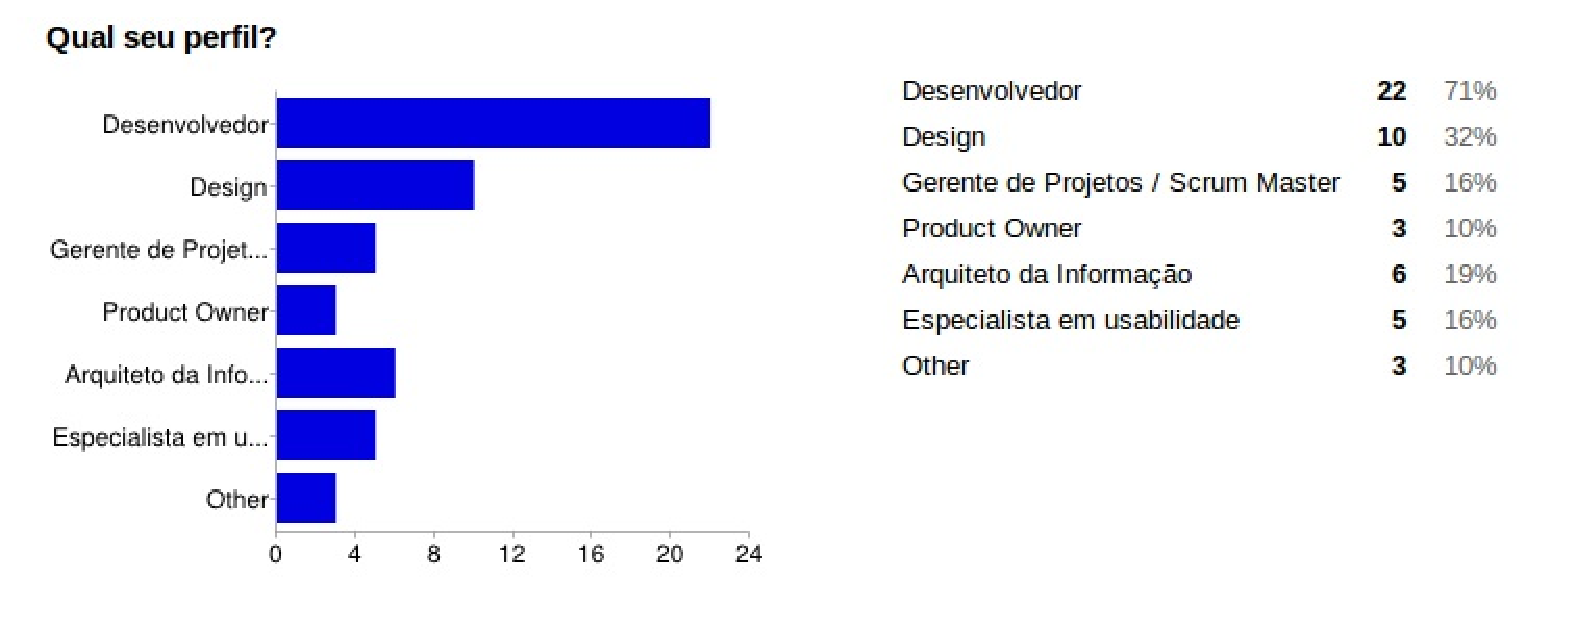
\includegraphics[keepaspectratio=true,scale=0.55]
      		{figuras/perfil.eps}
    	\label{concepcao}
		\caption{Perfil dos entrevistados}
	\end{figure}
	
	Como a pesquisa foi realizada com profissionais diversos, alguns não estavam envolvidos com software livre e com métodos ágeis simultâneamente. Dentre os pesquisados a grande maioria, 48\% tinham entre 1 e 2 anos de experiência com métodos ágeis. Em relação à software livre, 19\% entre 1 e 2 anos, 19\% de 5 a 10 anos e 19\% não trabalhavam com software livre.
	
	\begin{figure}[!h]
    	\centering
    	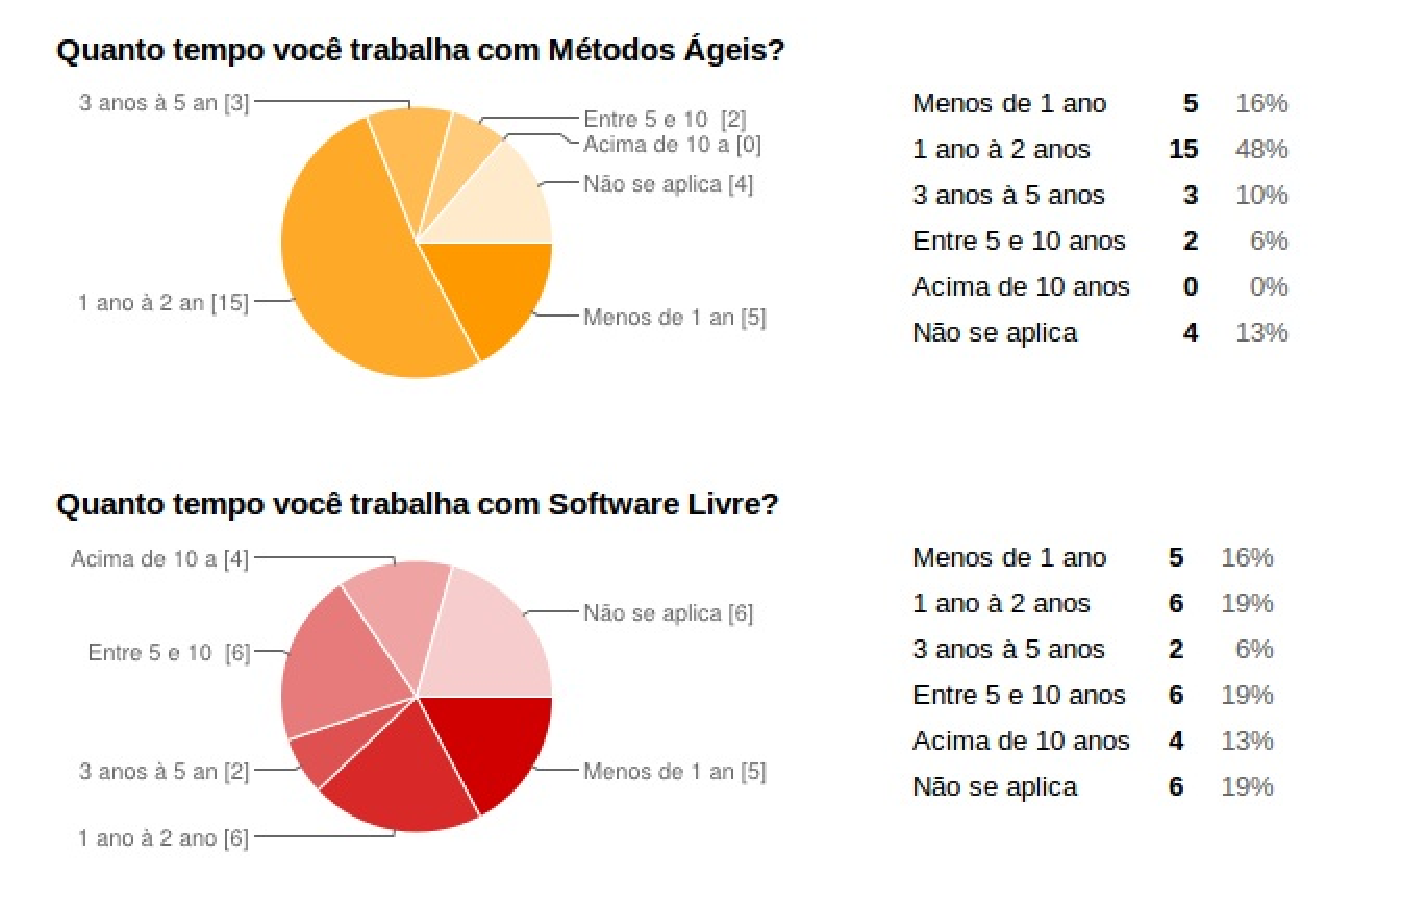
\includegraphics[keepaspectratio=true,scale=0.55]
      		{figuras/tempo_trabalho.eps}
    	\label{concepcao}
		\caption{Tempo de trabalho}
	\end{figure}			
	\begin{figure}[!h]
    	\centering
    	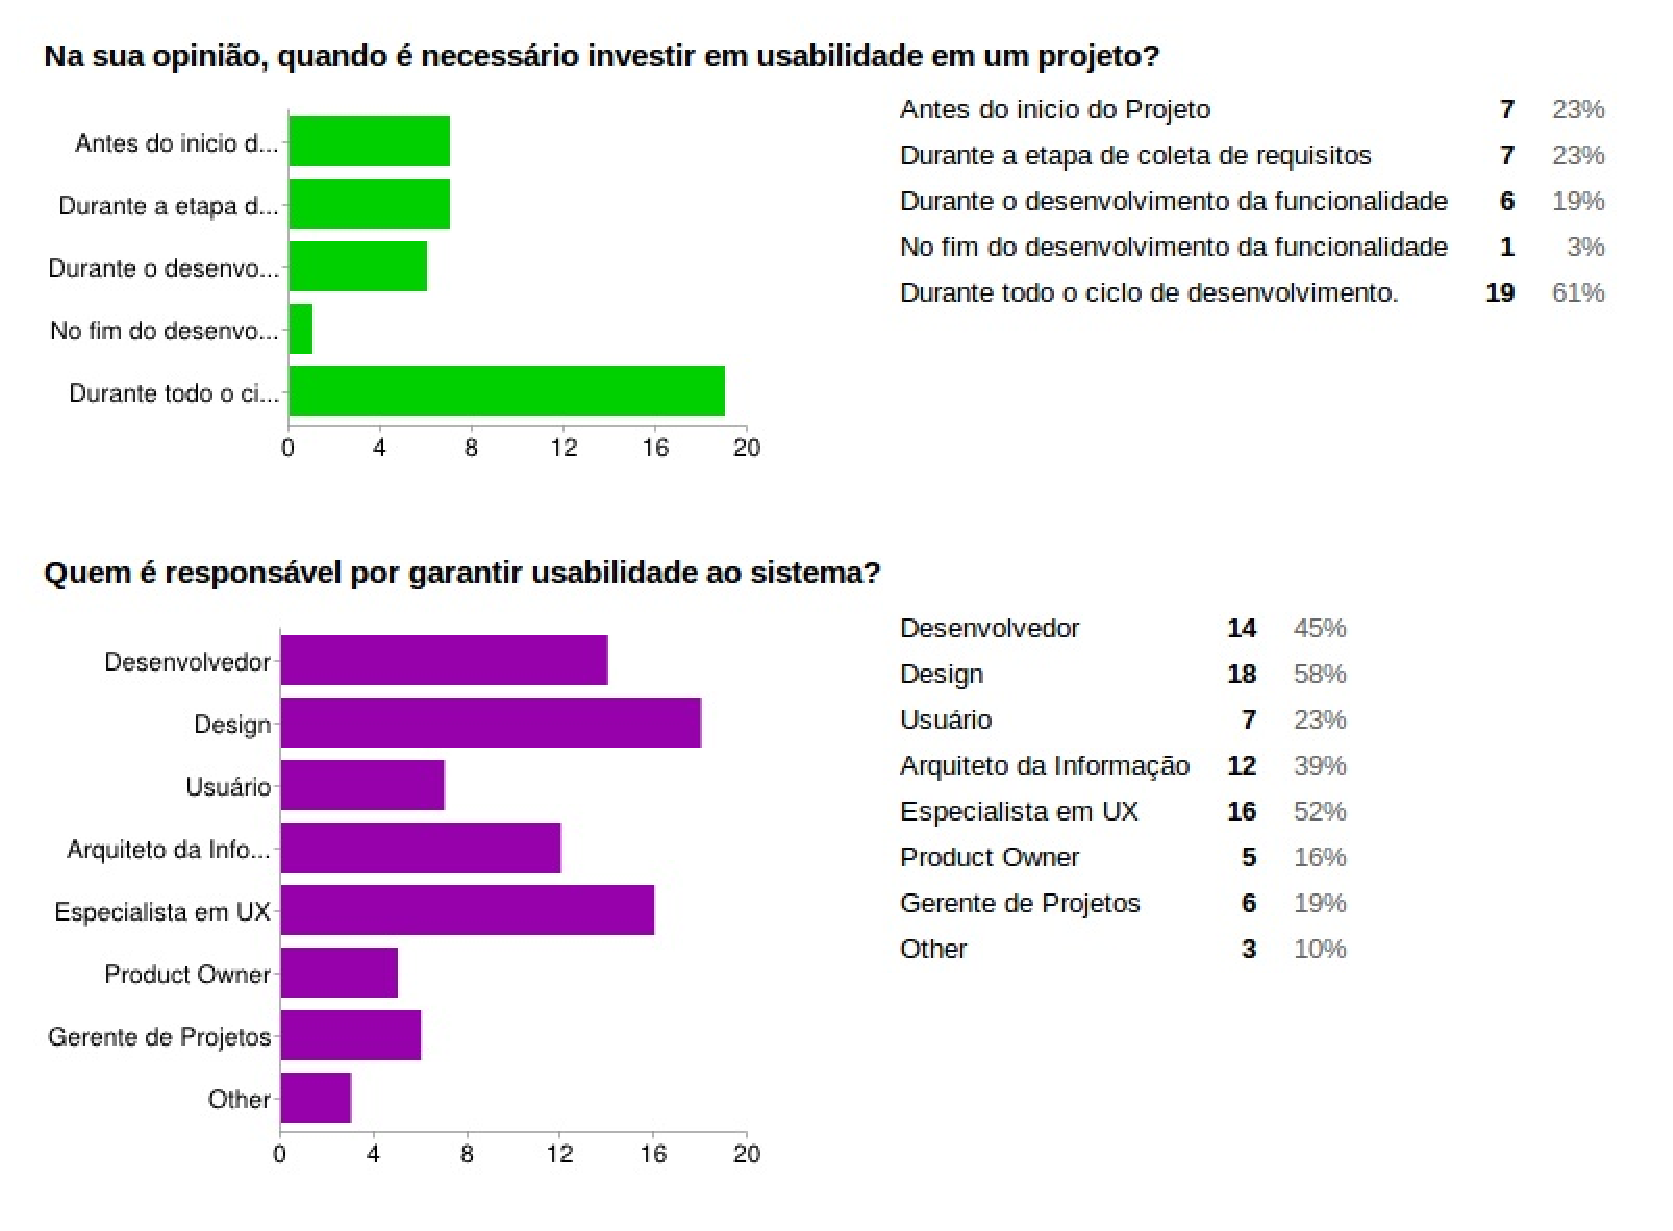
\includegraphics[keepaspectratio=true,scale=0.55]
      		{figuras/quando_e_quem.eps}
    	\label{concepcao}
		\caption{Quando e quem é responsável por garantir a usabilidade}
	\end{figure}

Para 61\% dos entrevistados, investir em usabilidade deve ser feito em todo o ciclo de desenvolvimento e realizada não somente pelos especialistas de usabilidade, mas também pelos desenvolvedores e designs.

\newpage

	Os resultados abaixo mostram as técnicas utilizadas pelos profissionais para avaliar, análisar e conceber interfaces com usabilidade.
	
	\begin{figure}[!h]
    	\centering
    	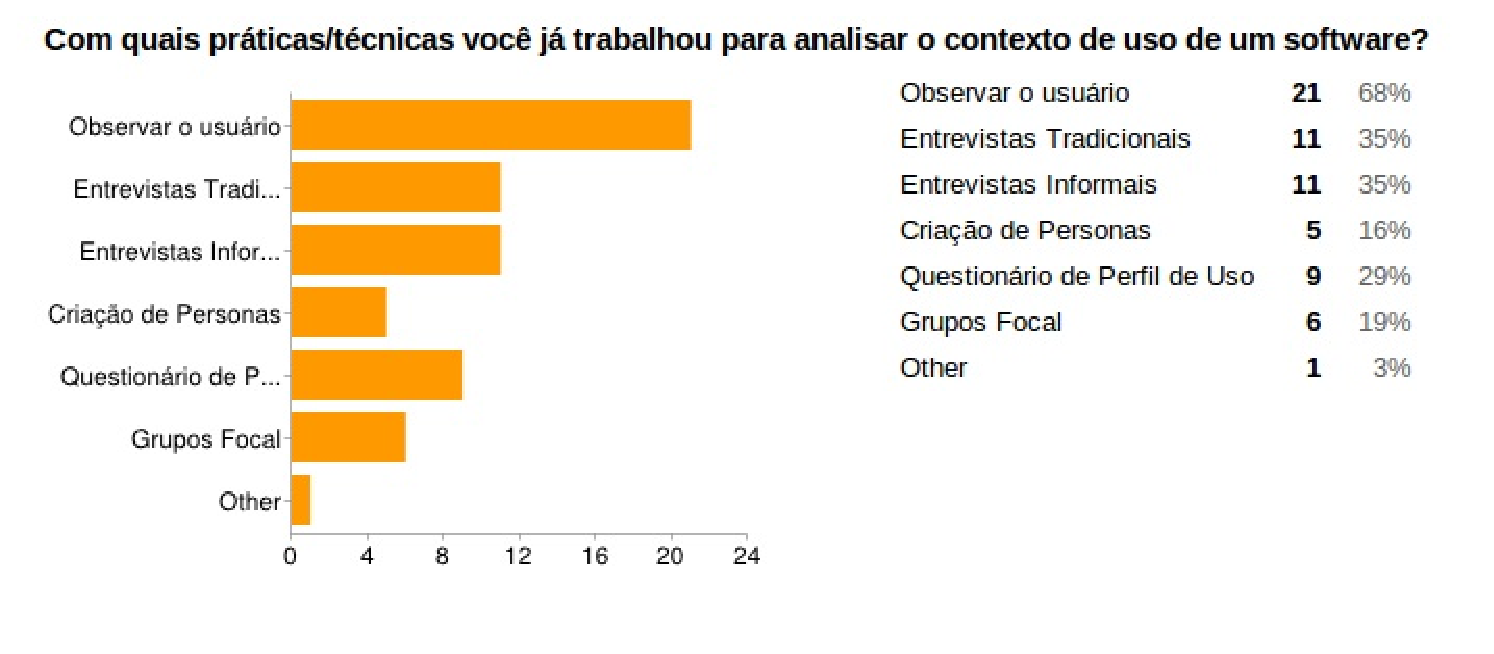
\includegraphics[keepaspectratio=true,scale=0.55]
      		{figuras/contexto_uso.eps}
    	\label{concepcao}
		\caption{Técnicas de contexto de uso}
	\end{figure}
	
	Uma das técnicas mais utilizadas para análisar o contexto de uso do sistema são as observações de usuários, com 68\%, as entrevistas estão em seguidas com 35\% e os questionários de perfil de uso com 29\%.
	
	\begin{figure}[!h]
    	\centering
    	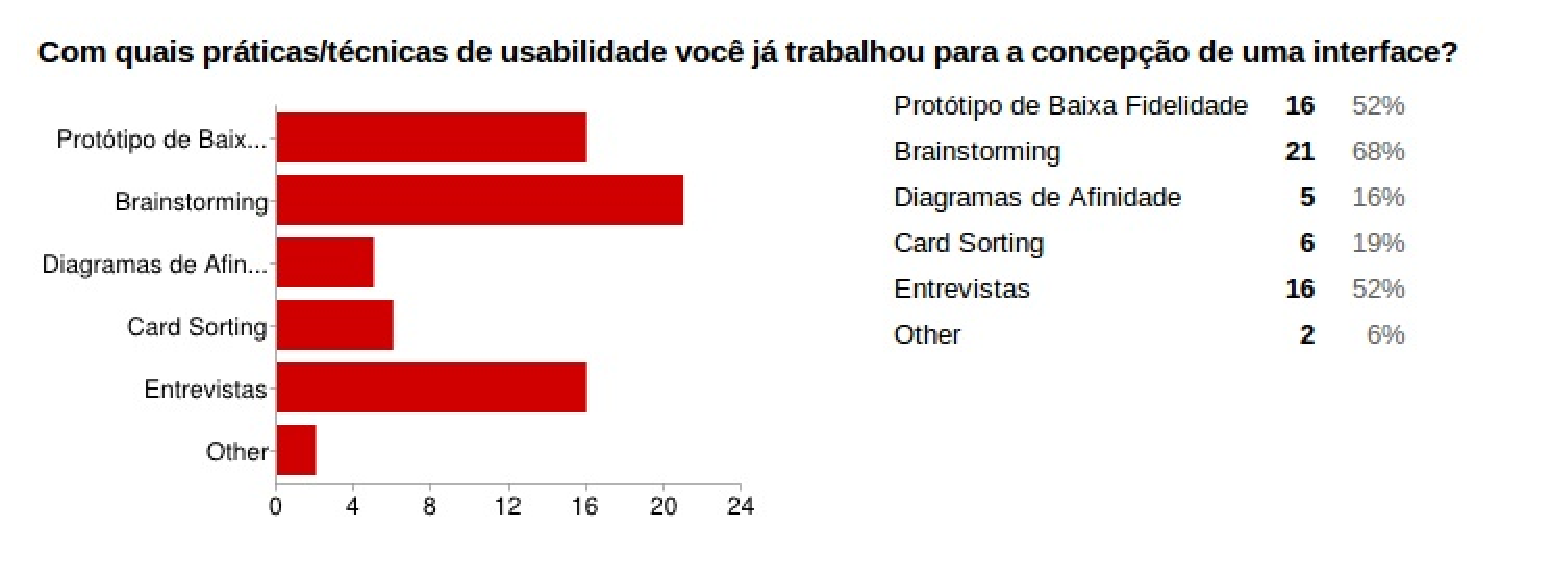
\includegraphics[keepaspectratio=true,scale=0.55]
      		{figuras/tecnica_concepcao.eps}
    	\label{concepcao}
		\caption{Técnicas de concepção de interfaces}
	\end{figure}
	
	A técnica de Braistorming é bastante utilizada por 68\% dos pesquisados para concepção de novas interfaces. Os protótipos de baixa fidelidade são bastante utilizados pelos pesquisados. 52\% também realizam entrevistas com usuários quando necessitam criar uma nova interface.
		
	\begin{figure}[!h]
    	\centering
    	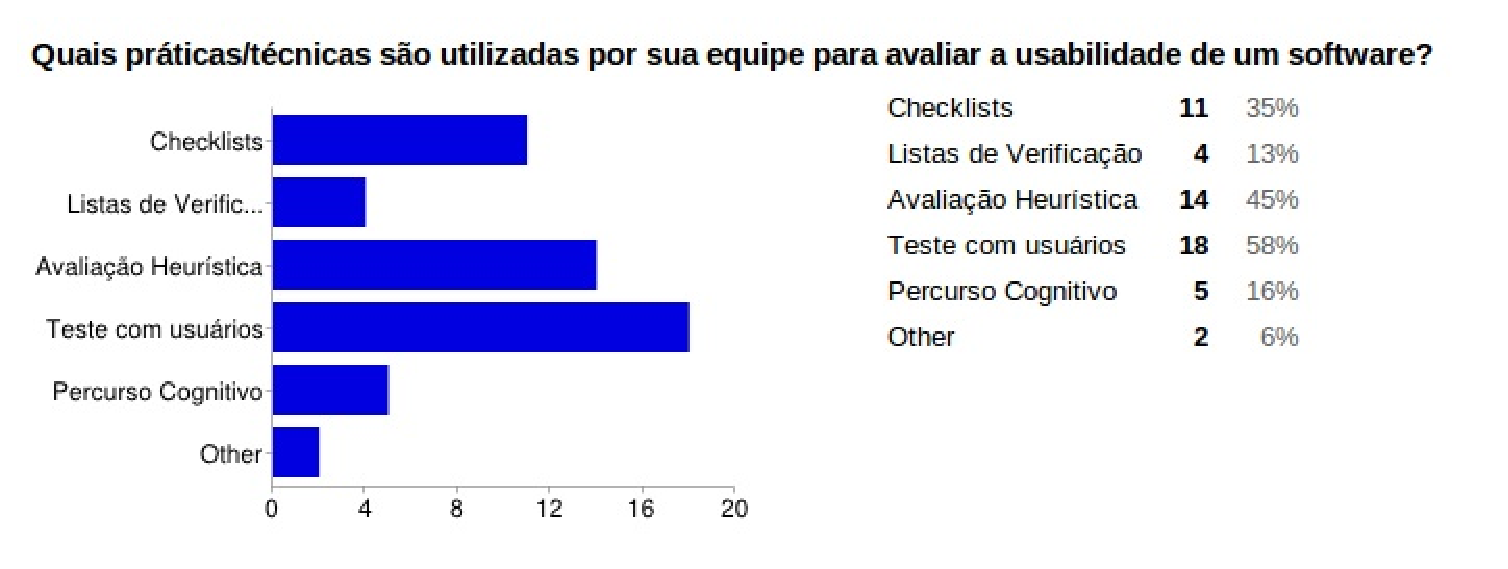
\includegraphics[keepaspectratio=true,scale=0.55]
      		{figuras/avaliacao_usada.eps}
    	\label{concepcao}
		\caption{Técnicas de avaliação utilizadas}
	\end{figure}	
	
	Os testes com usuários é uma das técnicas mais utilizadas pelos profissionais com 58\%, seguido pelas técnicas de avaliação heurísticas e checklists (listas de verificação). 
	
	Os resultados abaixo mostram qual a importância de cada técnica de concepção de uma interface de acordo com a percepção dos pesquisados.
	
	\begin{figure}[!h]
    	\centering
    	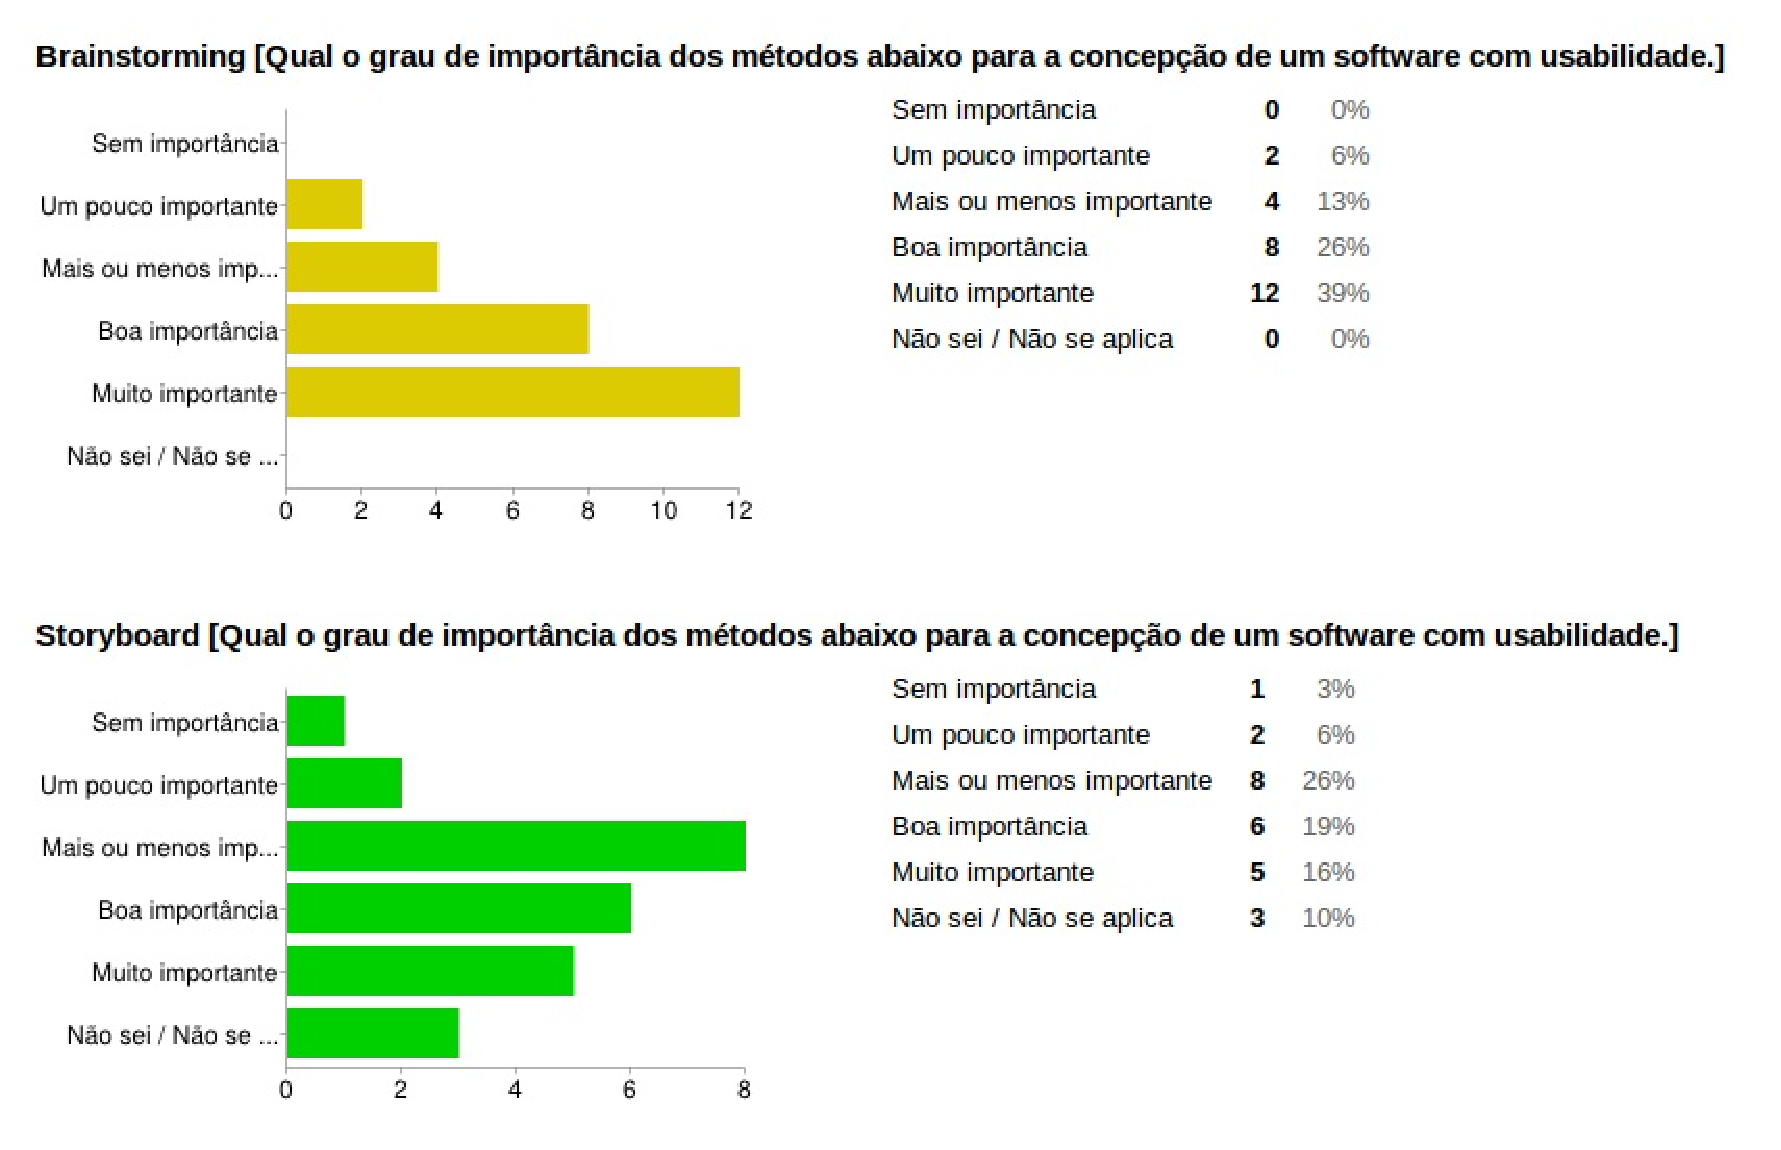
\includegraphics[keepaspectratio=true,scale=0.55]
      		{figuras/concepcao1.eps}
    	\label{concepcao}
		\caption{Técnicas de concepção - Brainstorming e Storyboard}
	\end{figure}
	
	Em relação ao Brainstorming, 39\% dos entrevistados concordam que a técnica é muito importante, já em relação ao storyboard a maioria, 26\% informa que é mais ou menos importante. 
	
	\begin{figure}[!h]
    	\centering
    	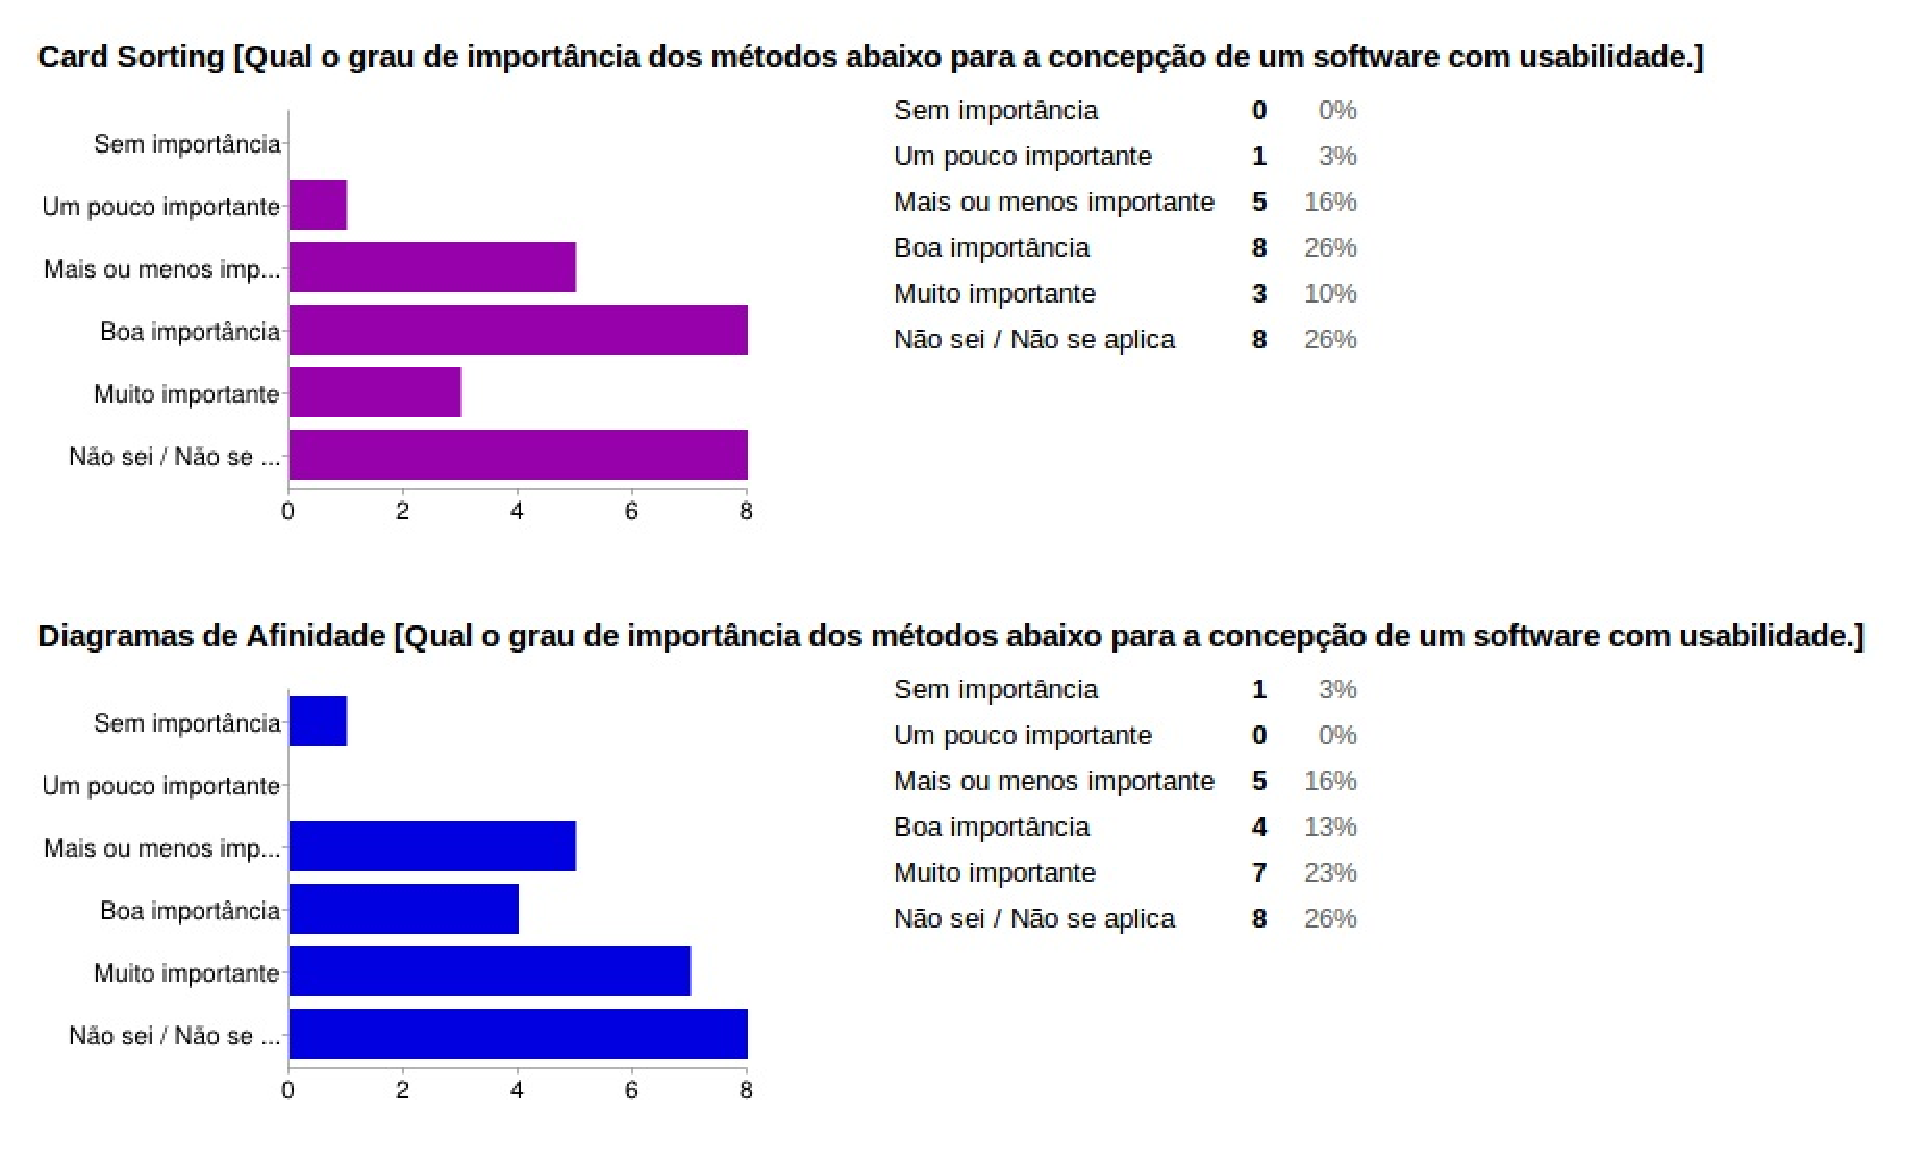
\includegraphics[keepaspectratio=true,scale=0.55]
      		{figuras/concepcao2.eps}
    	\label{check04}
		\caption{Técnicas de concepção - Card Sorting e Diagramas de Afinidade}
	\end{figure}

	Em relação as técnicas de Card Sorting e Diagramas de afinidade, 26 por cento dos pesquisados não sabiam o que eram cada técnica. 
		
	\begin{figure}[!h]
    	\centering
    	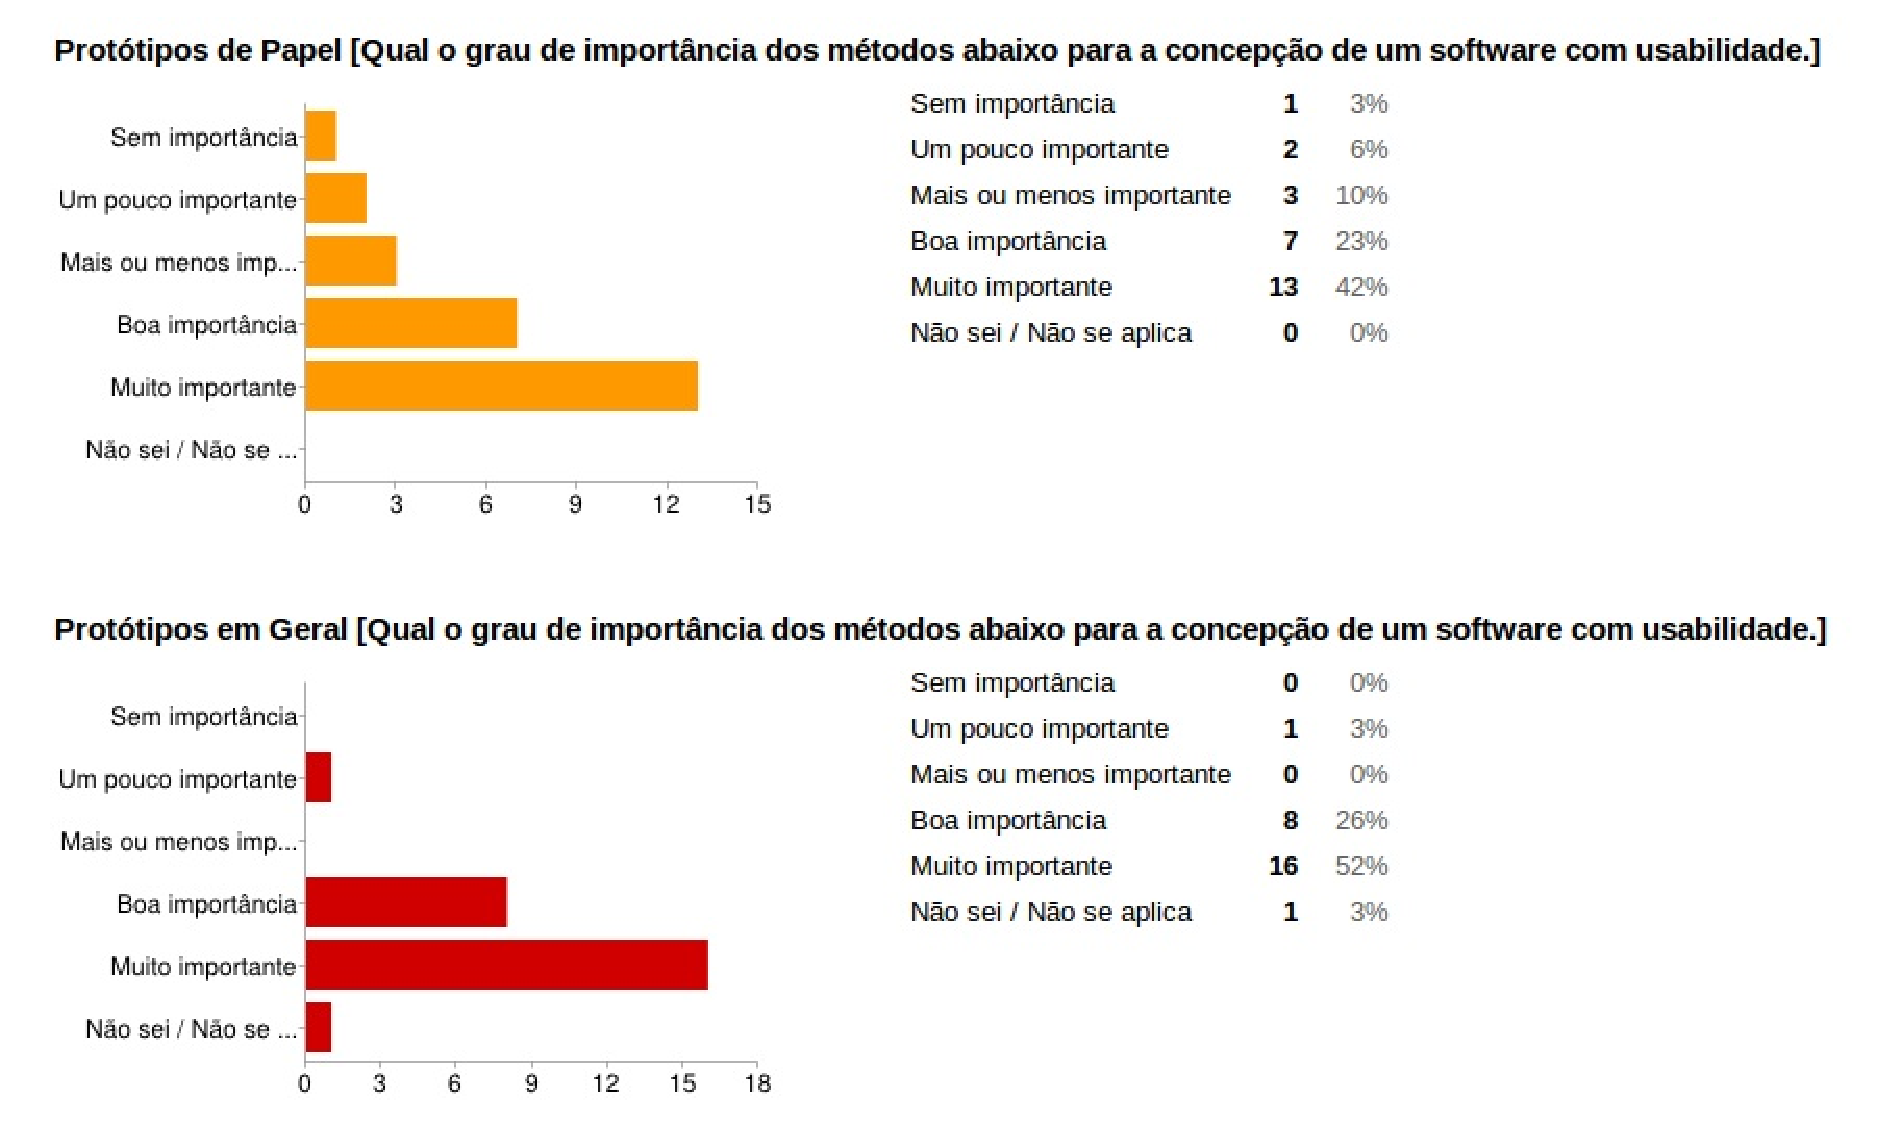
\includegraphics[keepaspectratio=true,scale=0.55]
      		{figuras/concepcao3.eps}
    	\label{check04}
		\caption{Técnicas de concepção - Protótipos}
	\end{figure}
	
	As técnicas de prototipação seja de baixa fidelidade ou geral obtiveram uma boa aceitação por parte dos pesquisados.

\newpage

	Os resultados abaixo mostram a importância das técnicas de análise.
	
	\begin{figure}[!h]
    	\centering
    	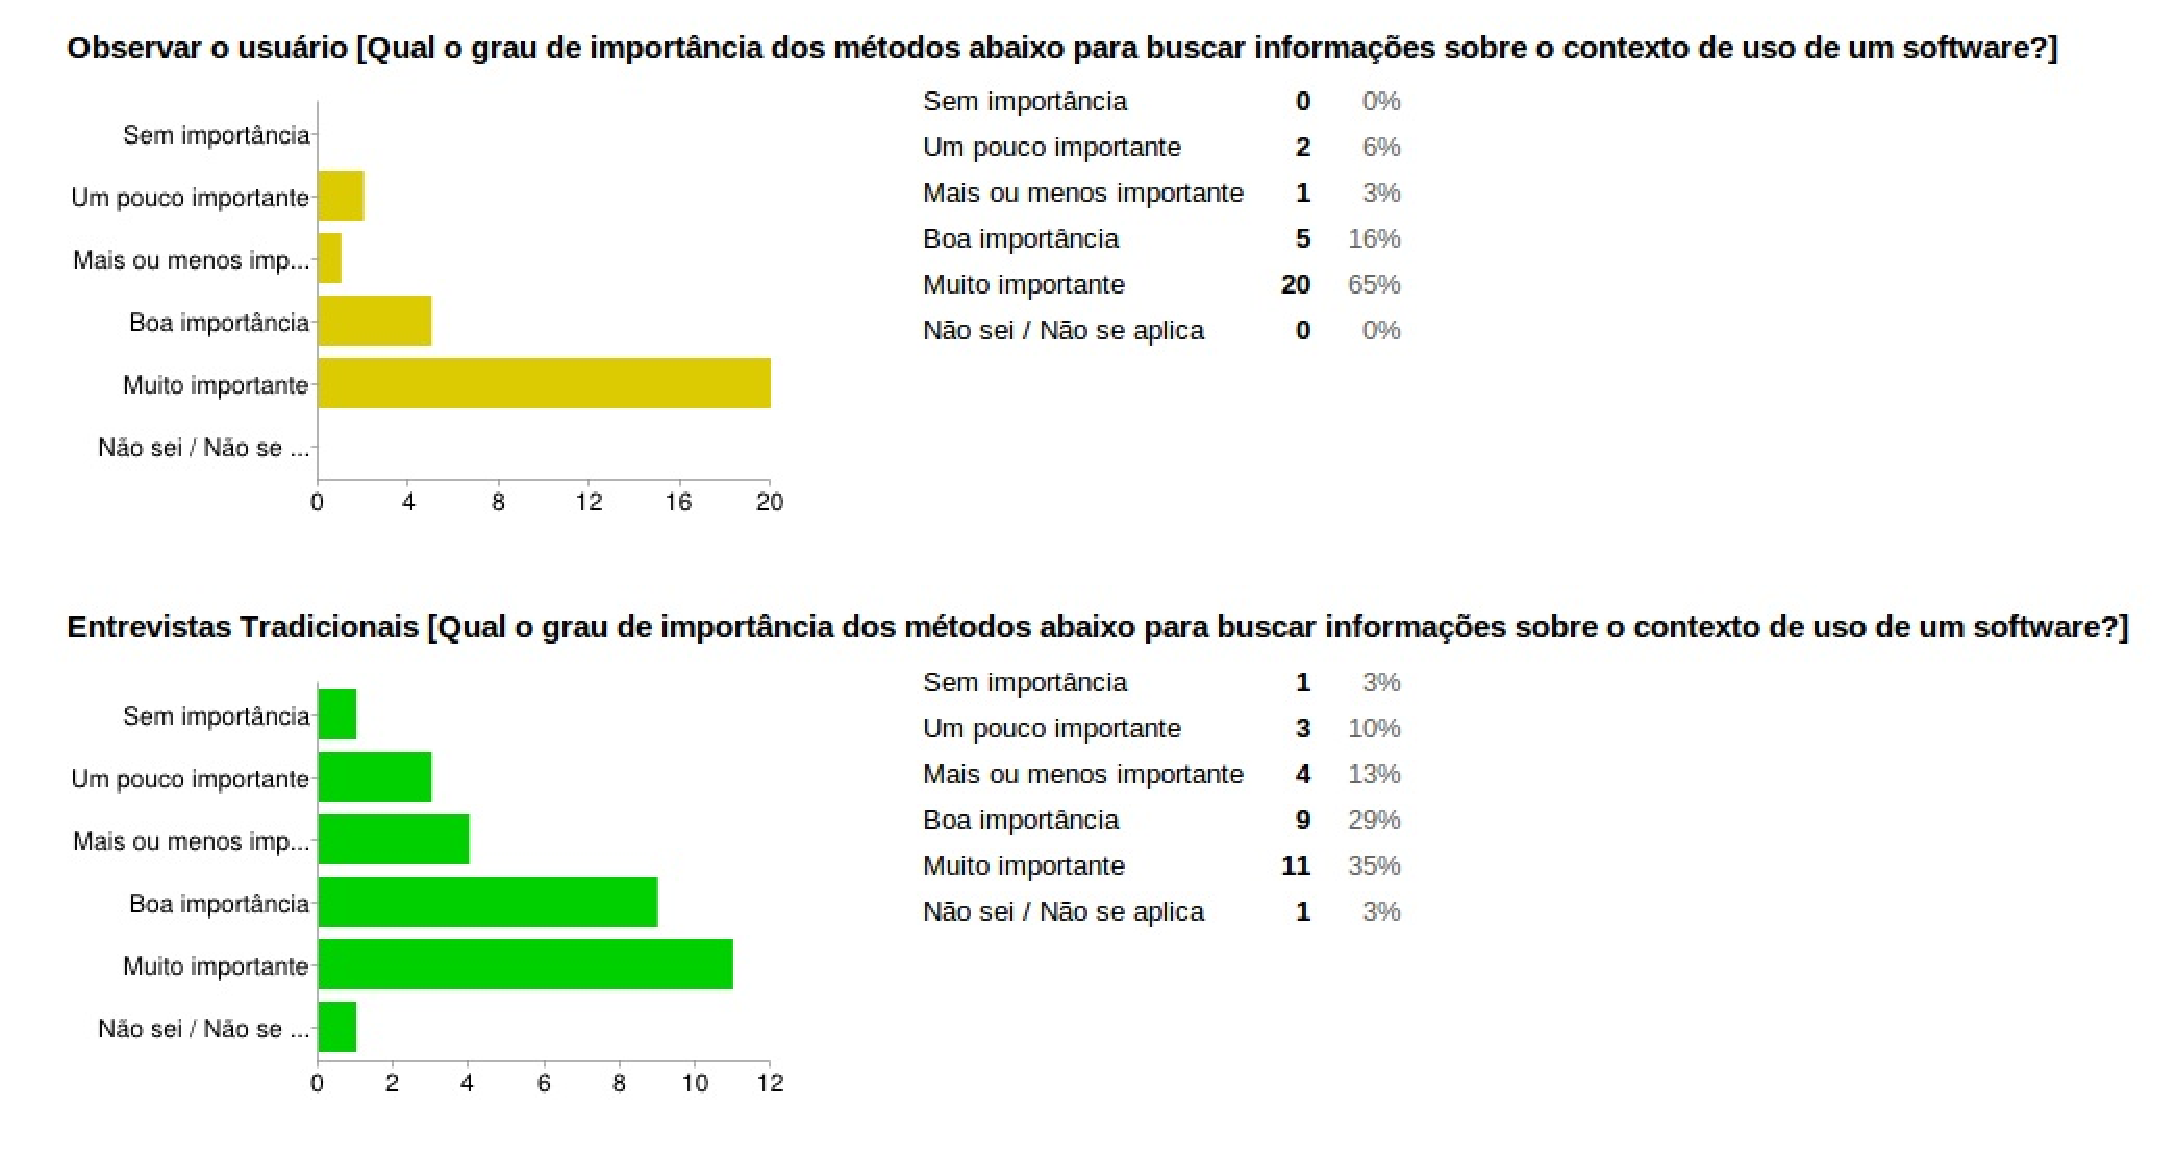
\includegraphics[keepaspectratio=true,scale=0.50]
      		{figuras/analise1.eps}
    	\label{check04}
		\caption{Técnicas de análise - Observação e entrevistas tradicionais}
	\end{figure}
	
	As técnica de observar o usuário obteve uma grande aceitação por parte dos pesquisados, sendo 65\% tendo muita importância.
	 
	As entrevistas tanto tradicionais, como as informais obtiveram resultados pŕoximos, mais de 50\% informaram que têm boa ou muita importância.
		
	\begin{figure}[!h]
    	\centering
    	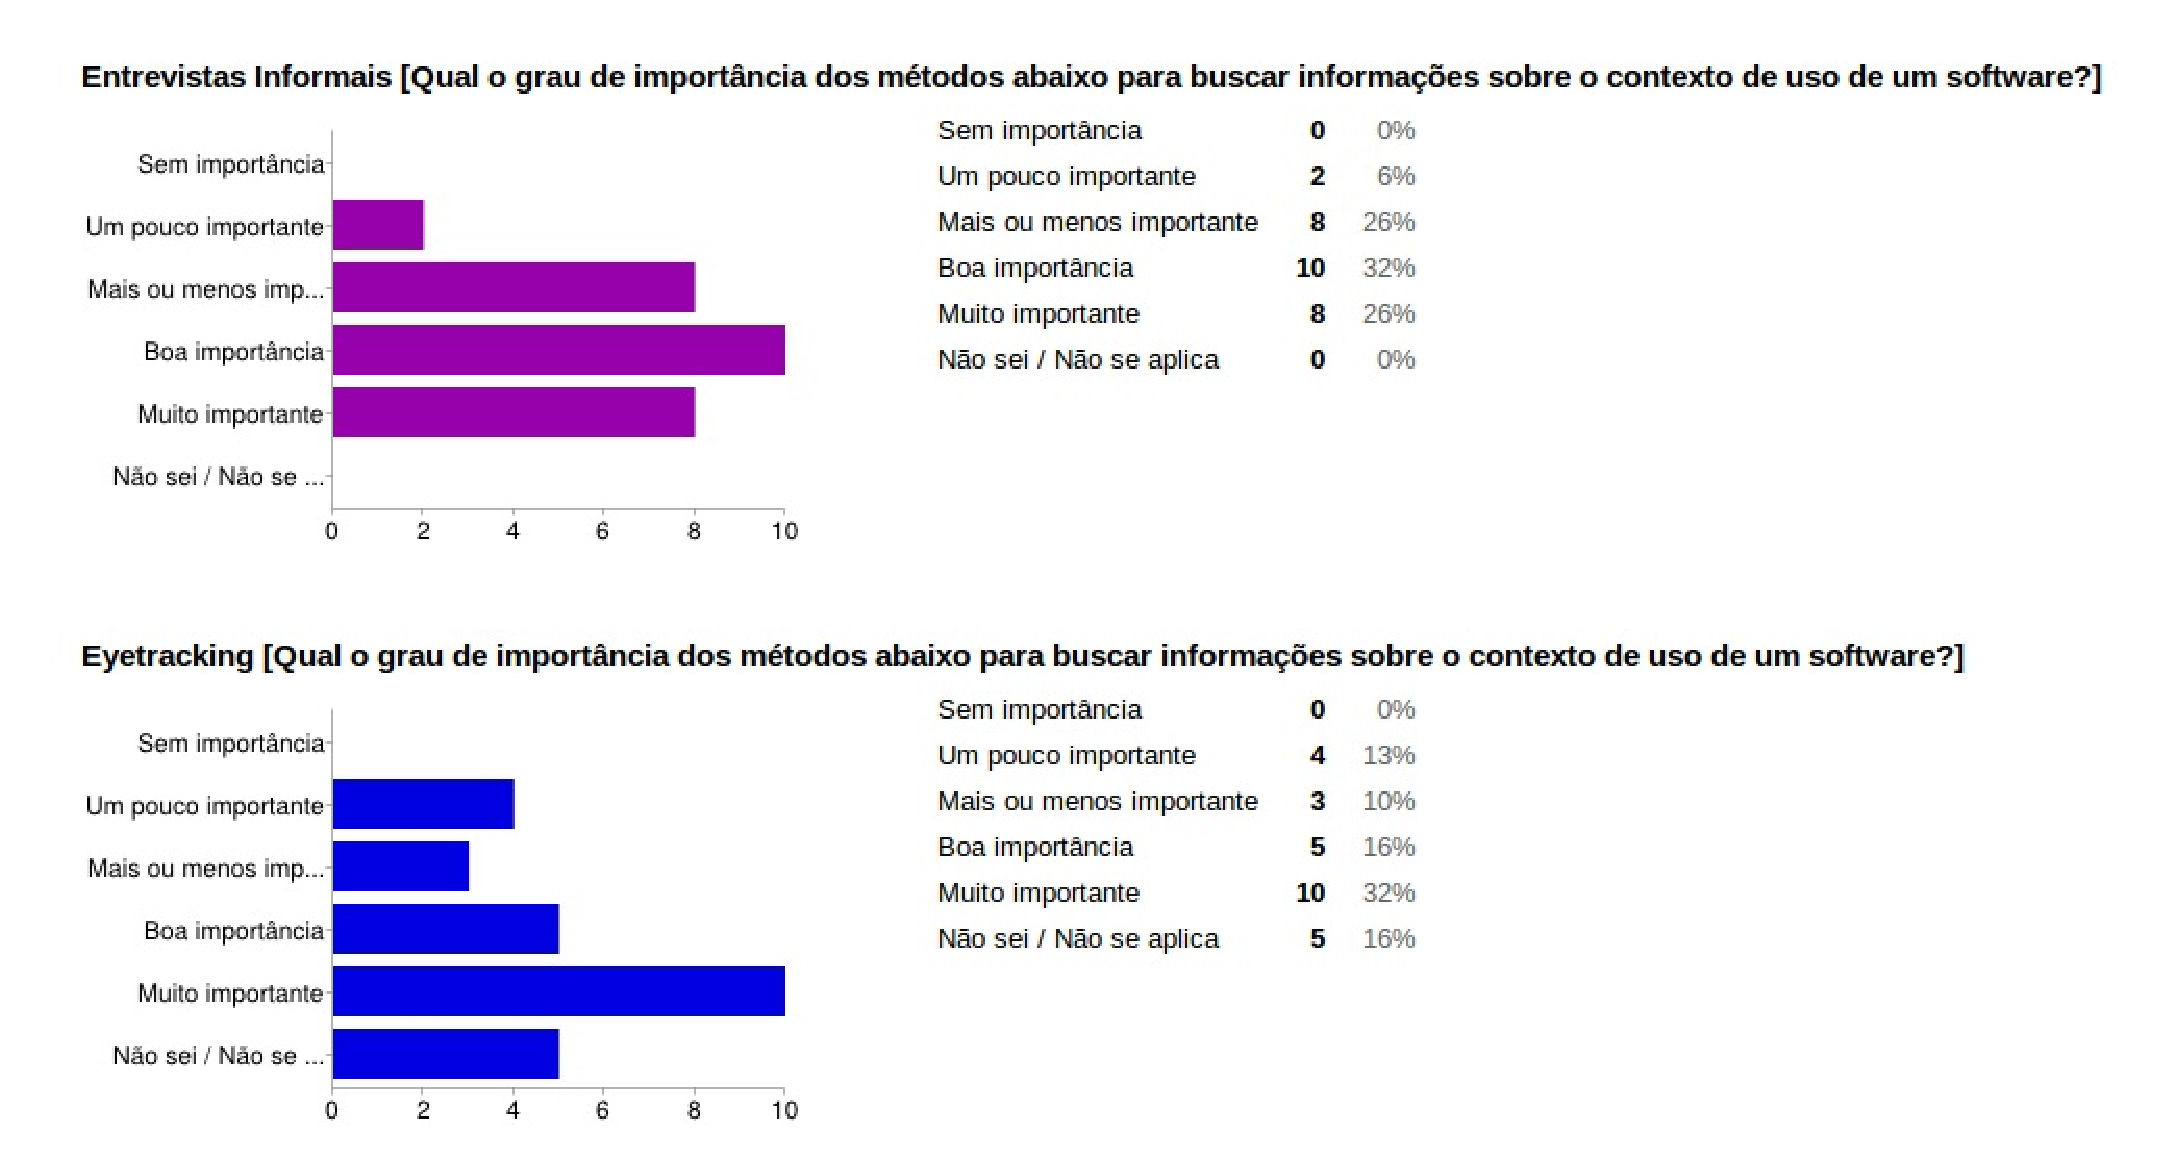
\includegraphics[keepaspectratio=true,scale=0.50]
      		{figuras/analise2.eps}
    	\label{check04}
		\caption{Técnicas de análise - Entrevistas Informais e Eytracking}
	\end{figure}

	32\% dos pesquisados informaram que a técnica de Eytracking é muito importante e 16\% não sabiam ou não aplicavam tal técnica.
		
	\begin{figure}[!h]
    	\centering
    	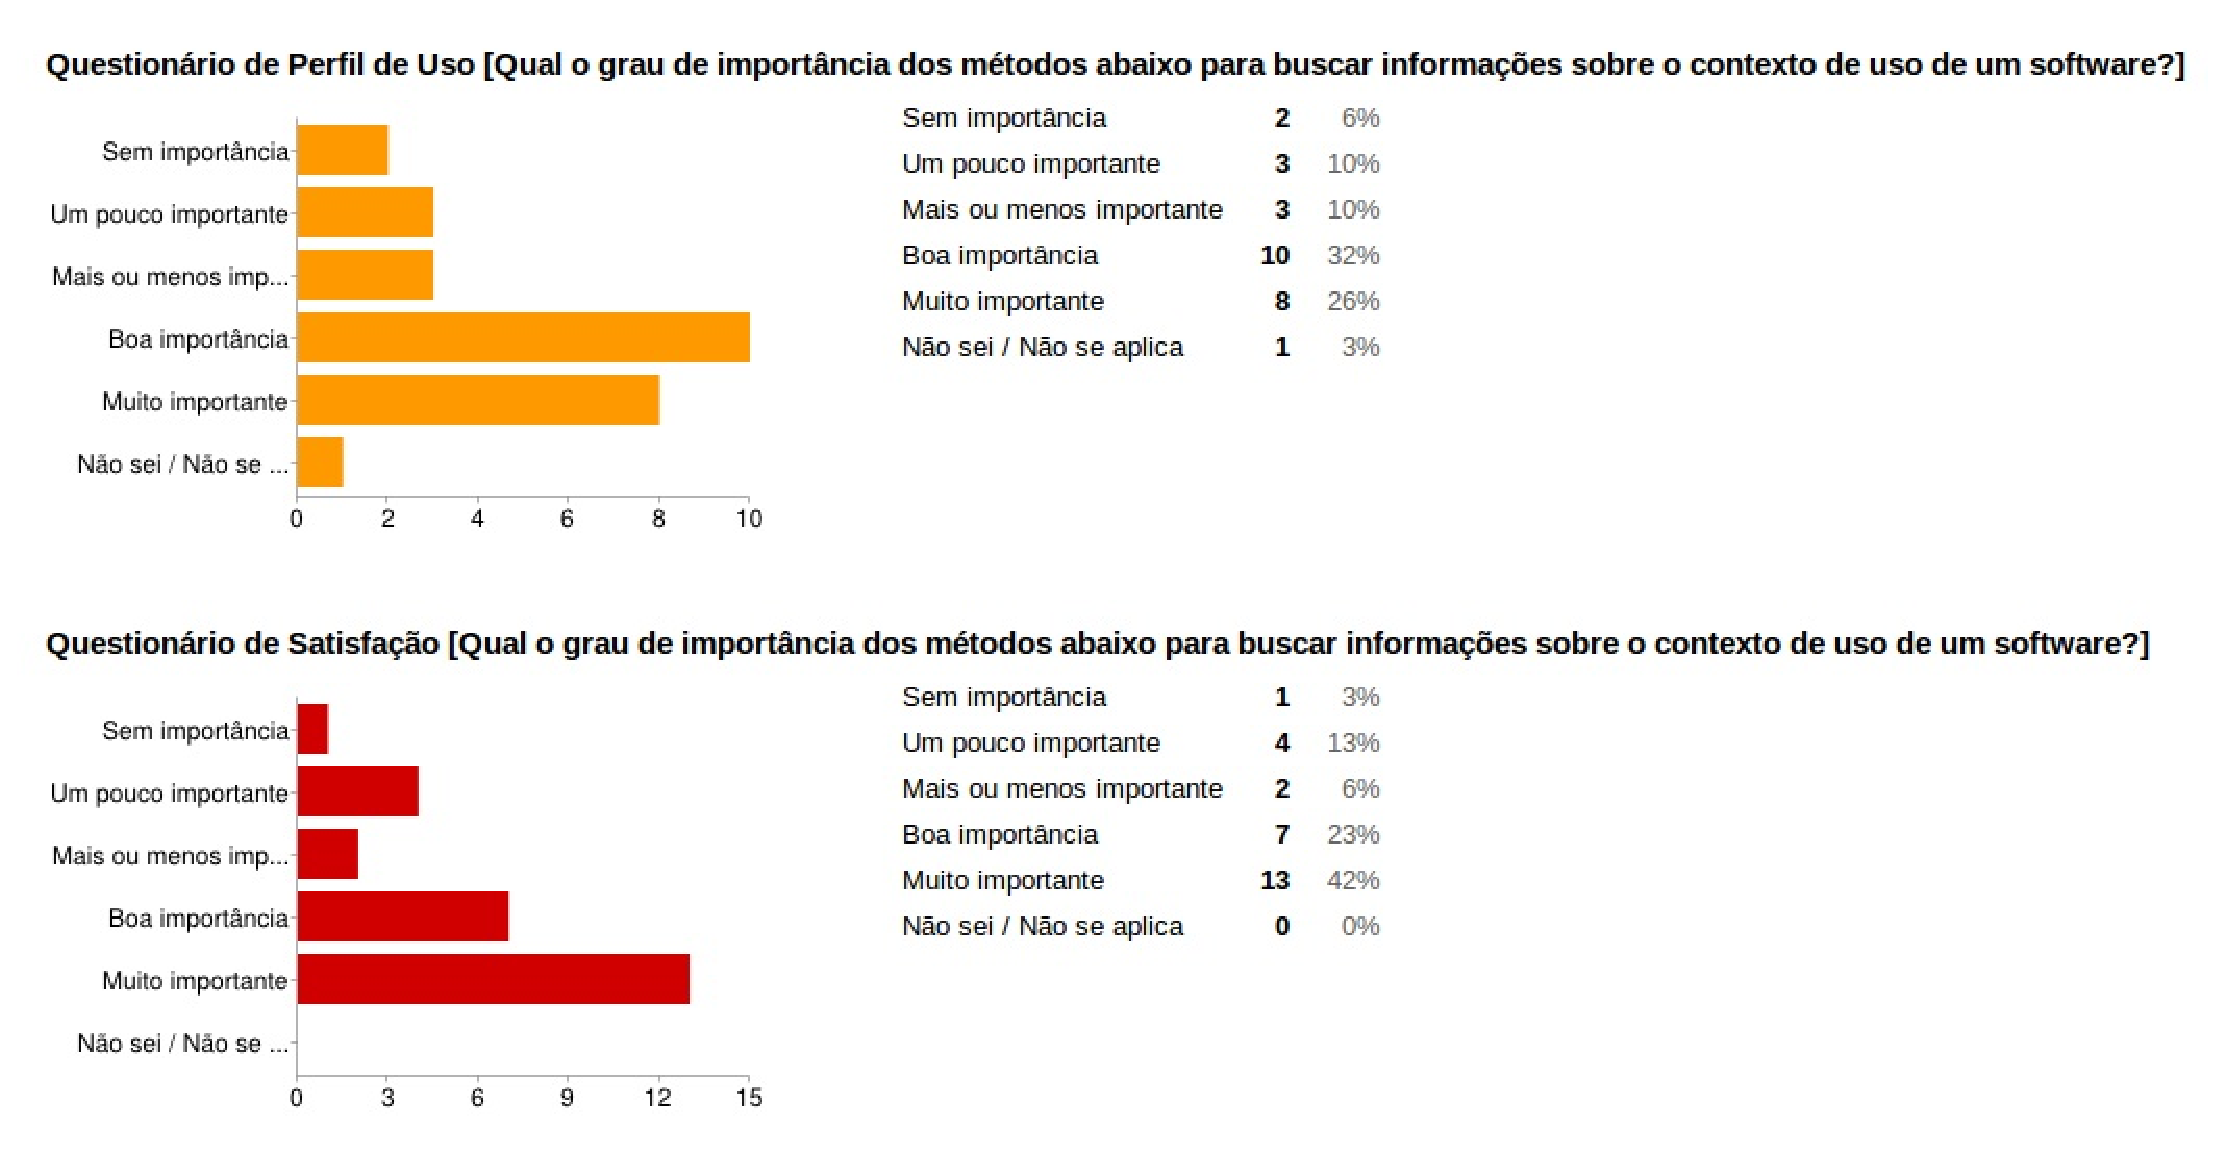
\includegraphics[keepaspectratio=true,scale=0.50]
      		{figuras/analise3.eps}
    	\label{check04}
		\caption{Técnicas de análise 'Questionários de perfil de uso e de satisfação}
	\end{figure}
	
	Os questionários de perfil de uso obtiveram boa importância, 32\%, mas alguns pesquisados, 6\% informaram que não são muito importante para realização de análises no contexto que estão inseridos.
	
	\begin{figure}[!h]
    	\centering
    	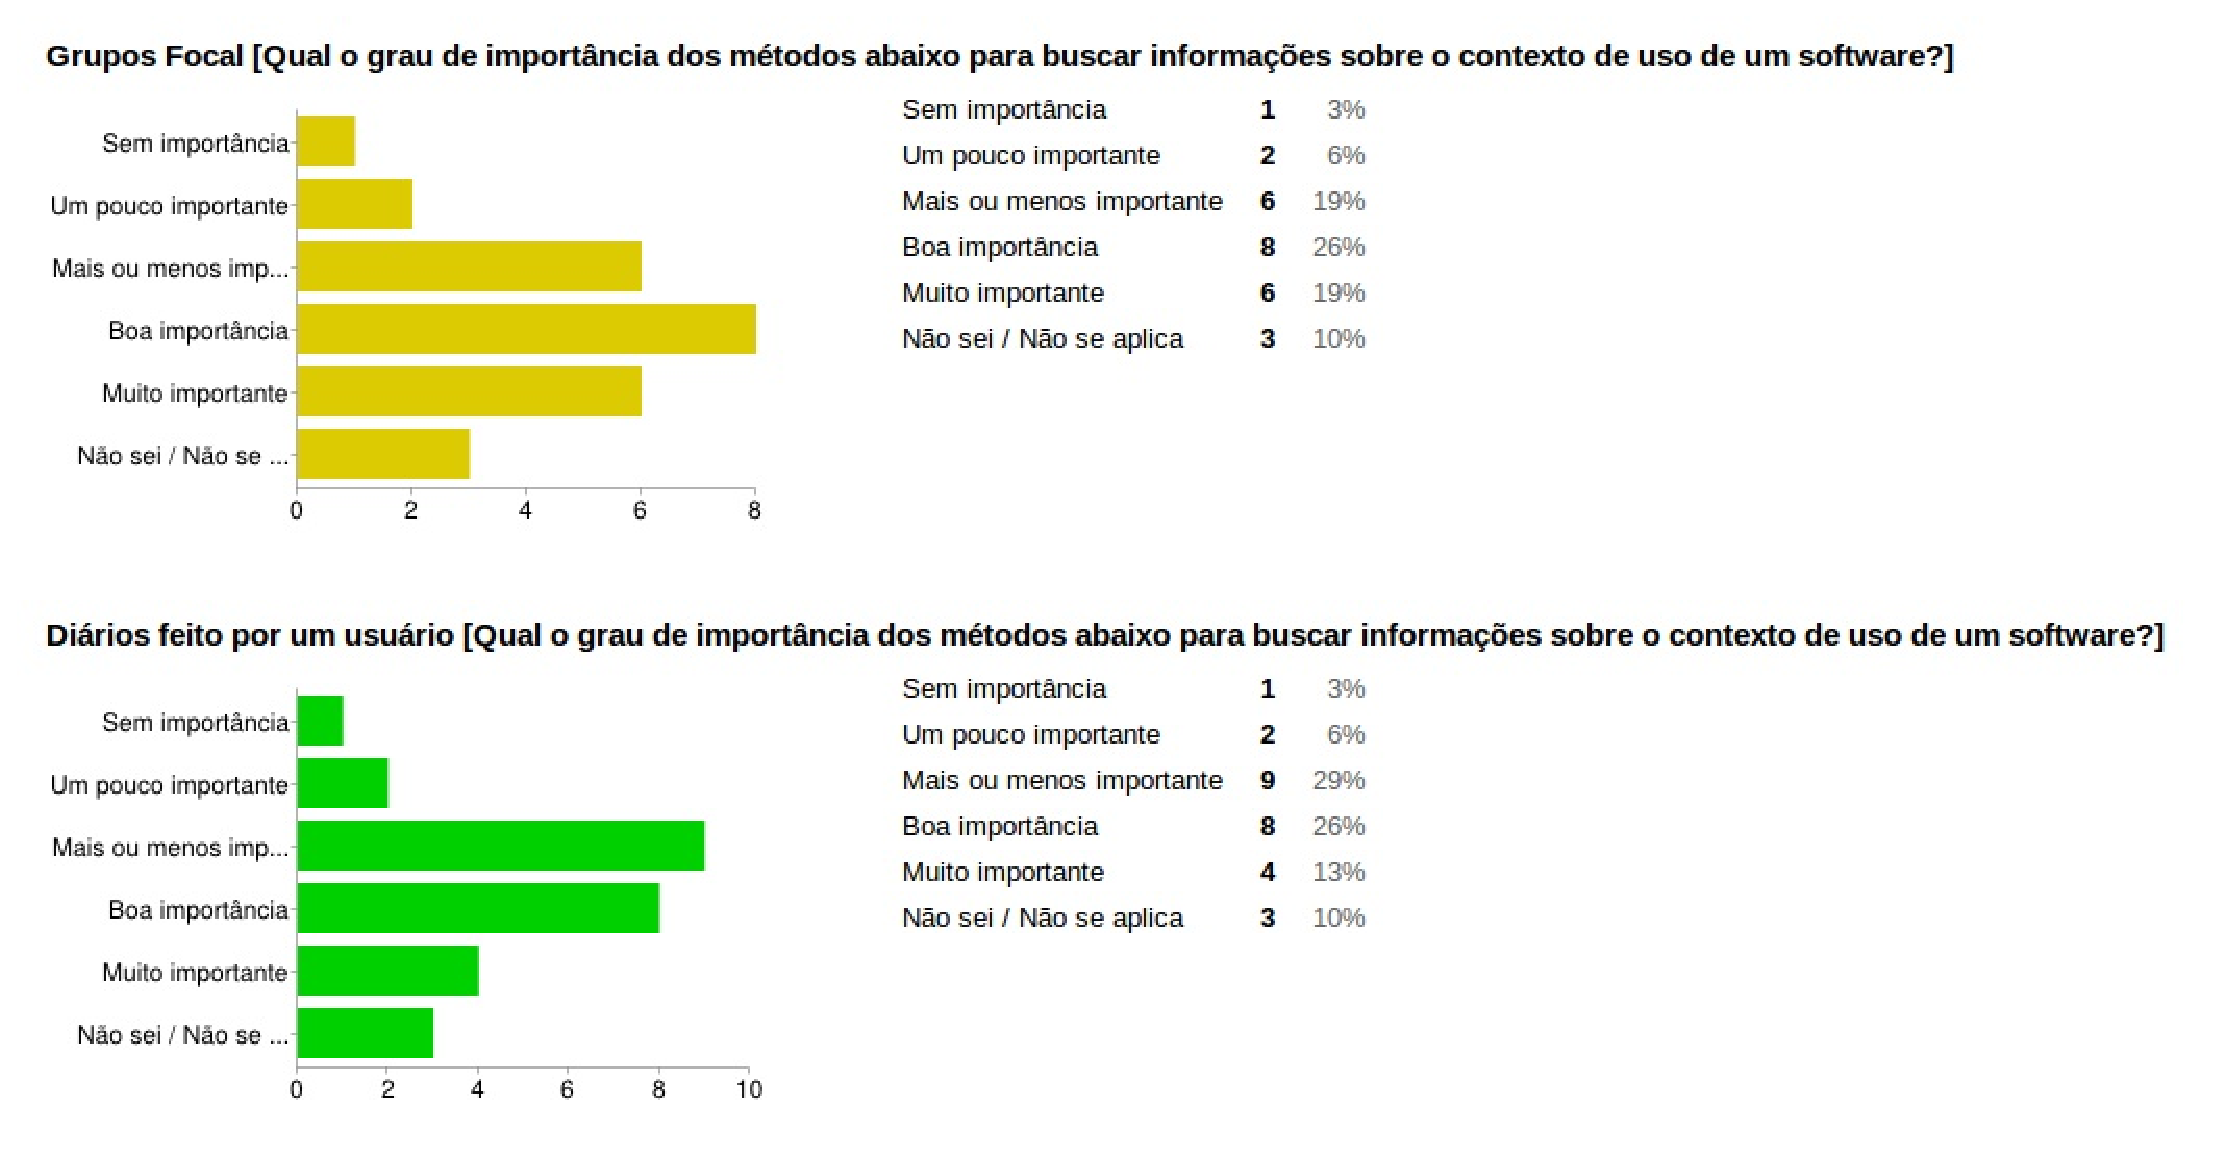
\includegraphics[keepaspectratio=true,scale=0.50]
      		{figuras/analise4.eps}
    	\label{check04}
		\caption{Técnicas de análise - Grupo Focal e Diários}
	\end{figure}
	
	
	\begin{figure}[!h]
    	\centering
    	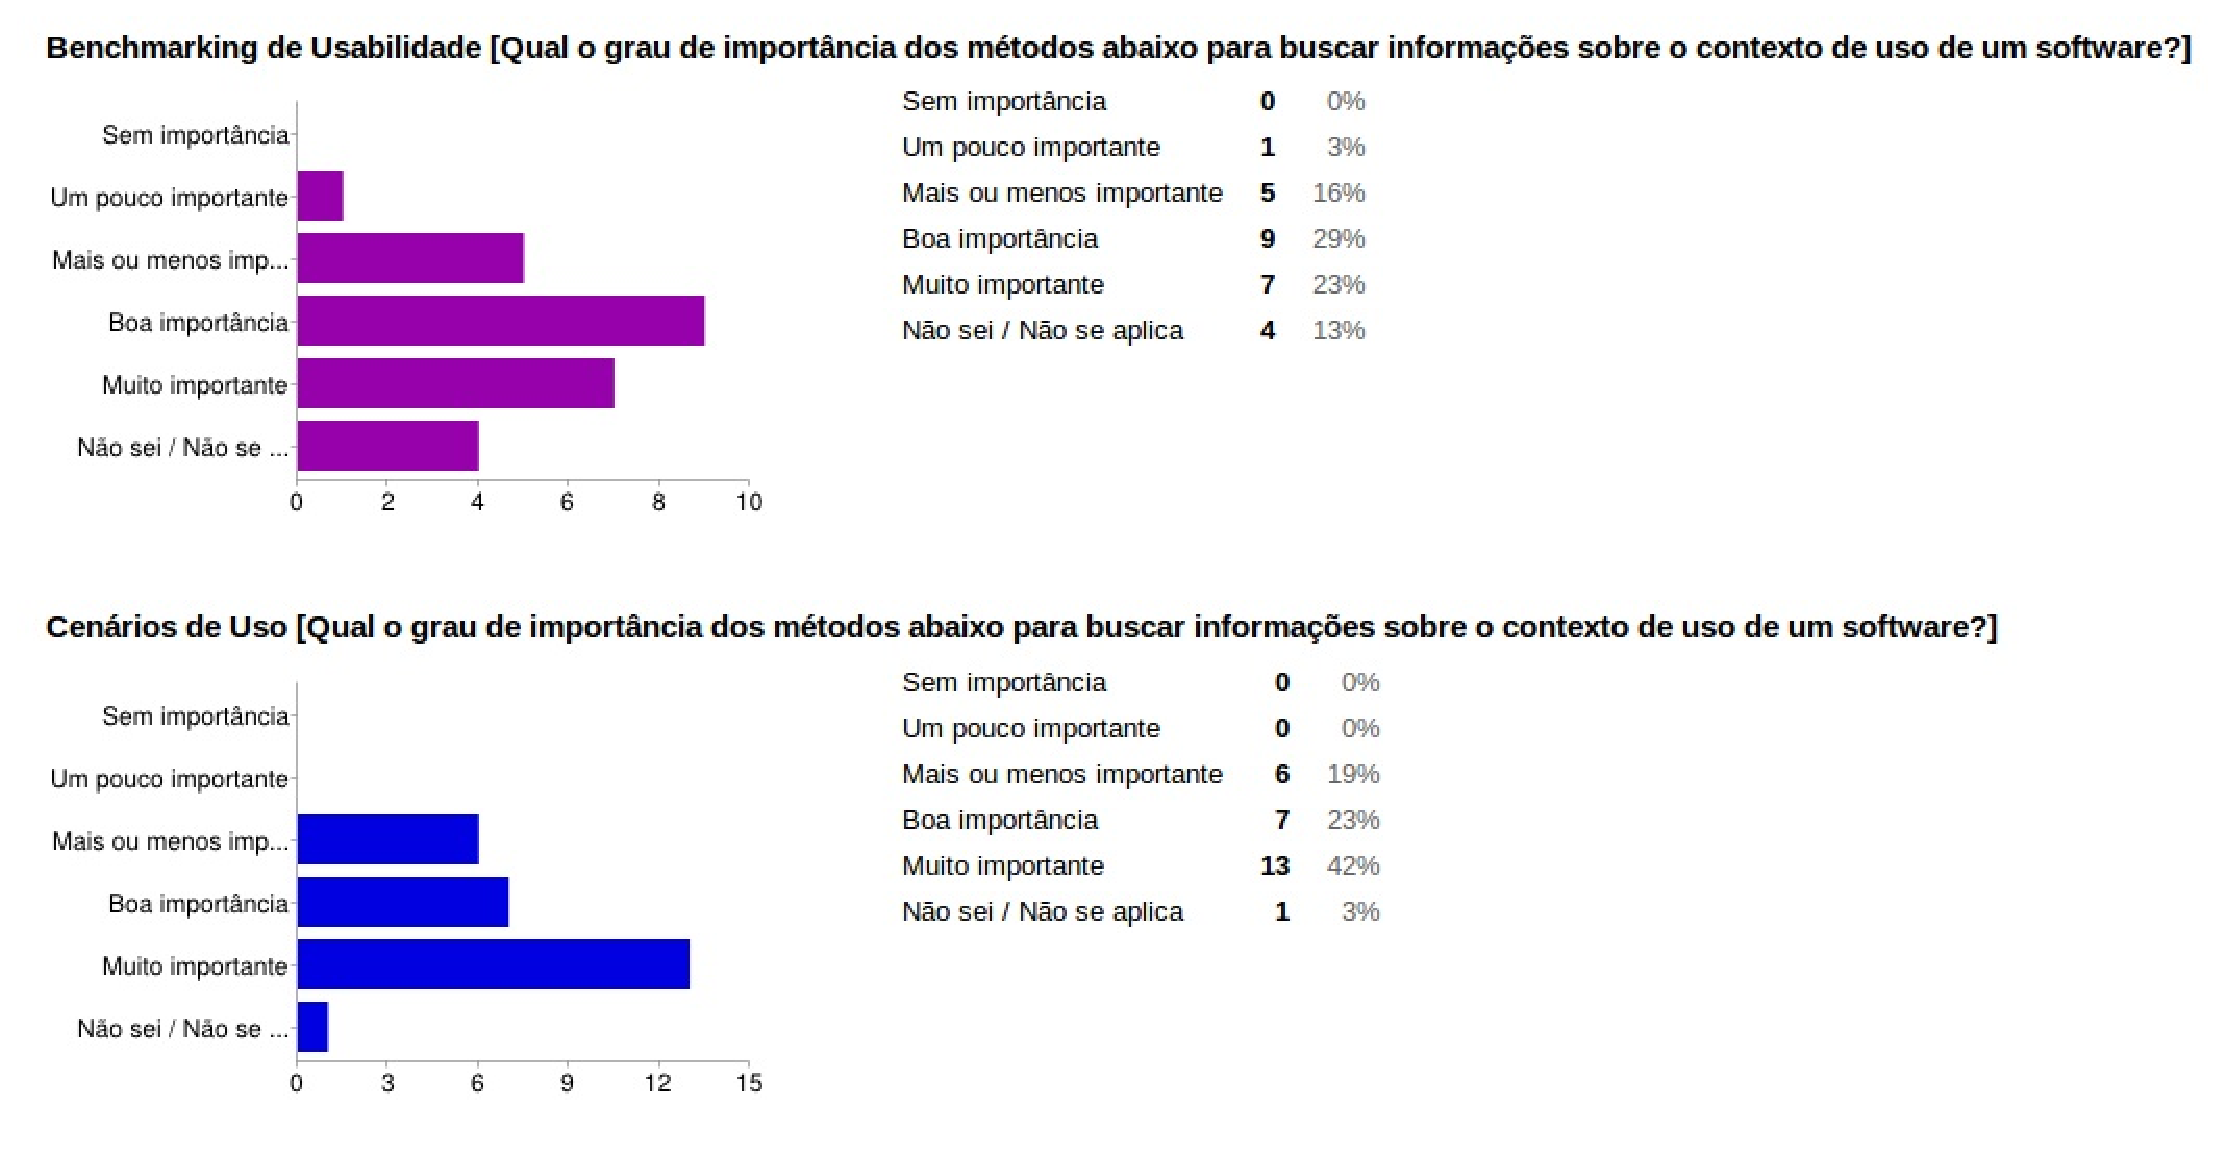
\includegraphics[keepaspectratio=true,scale=0.50]
      		{figuras/analise5.eps}
    	\label{check04}
		\caption{Técnicas de análise - Benchmarking e Cenários de uso}
	\end{figure}
		
	\begin{figure}[!h]
    	\centering
    	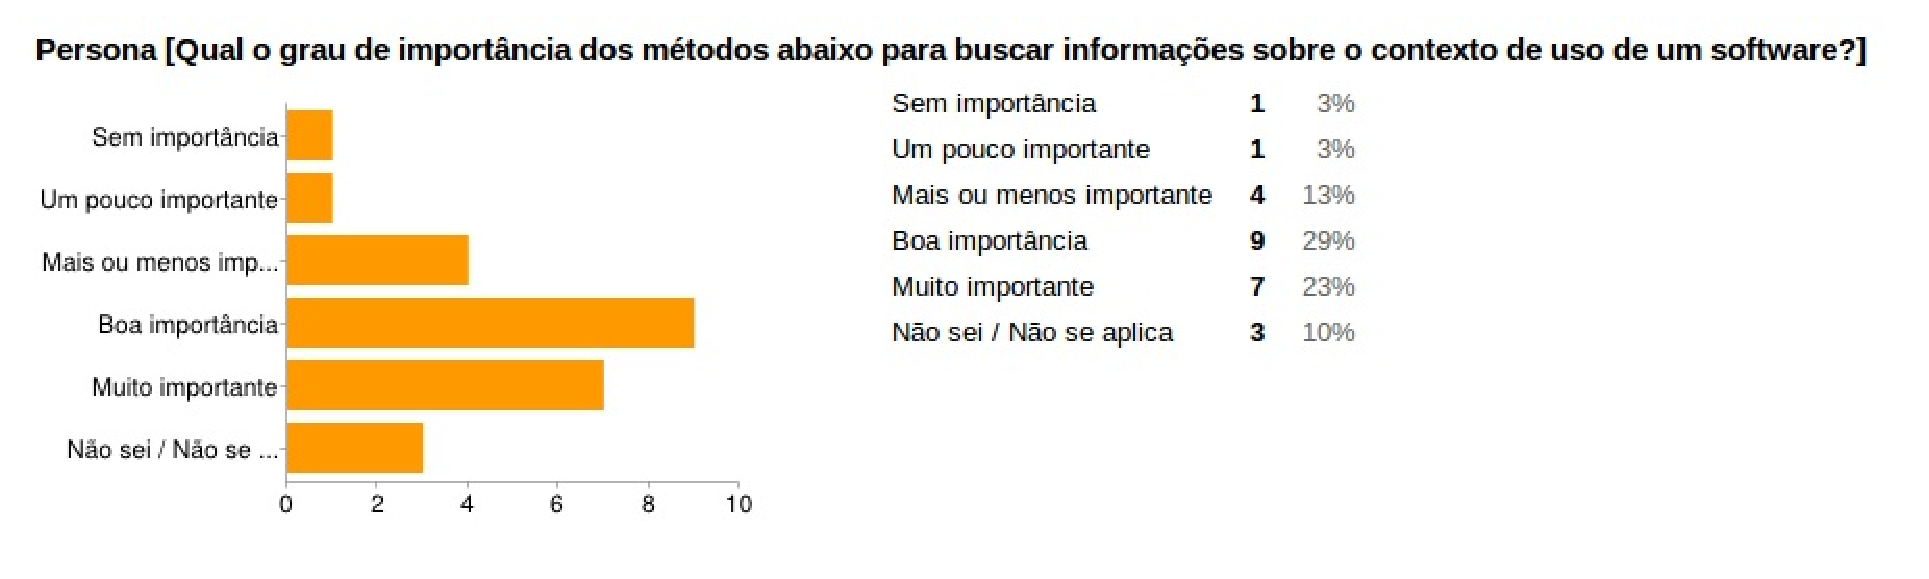
\includegraphics[keepaspectratio=true,scale=0.55]
      		{figuras/analise6.eps}
    	\label{check04}
		\caption{Técnicas de análise - Persona}
	\end{figure}

\newpage

	Os resultados abaixo são referentes as técnicas de avaliação da usabilidade.	
	
	\begin{figure}[!h]
    	\centering
    	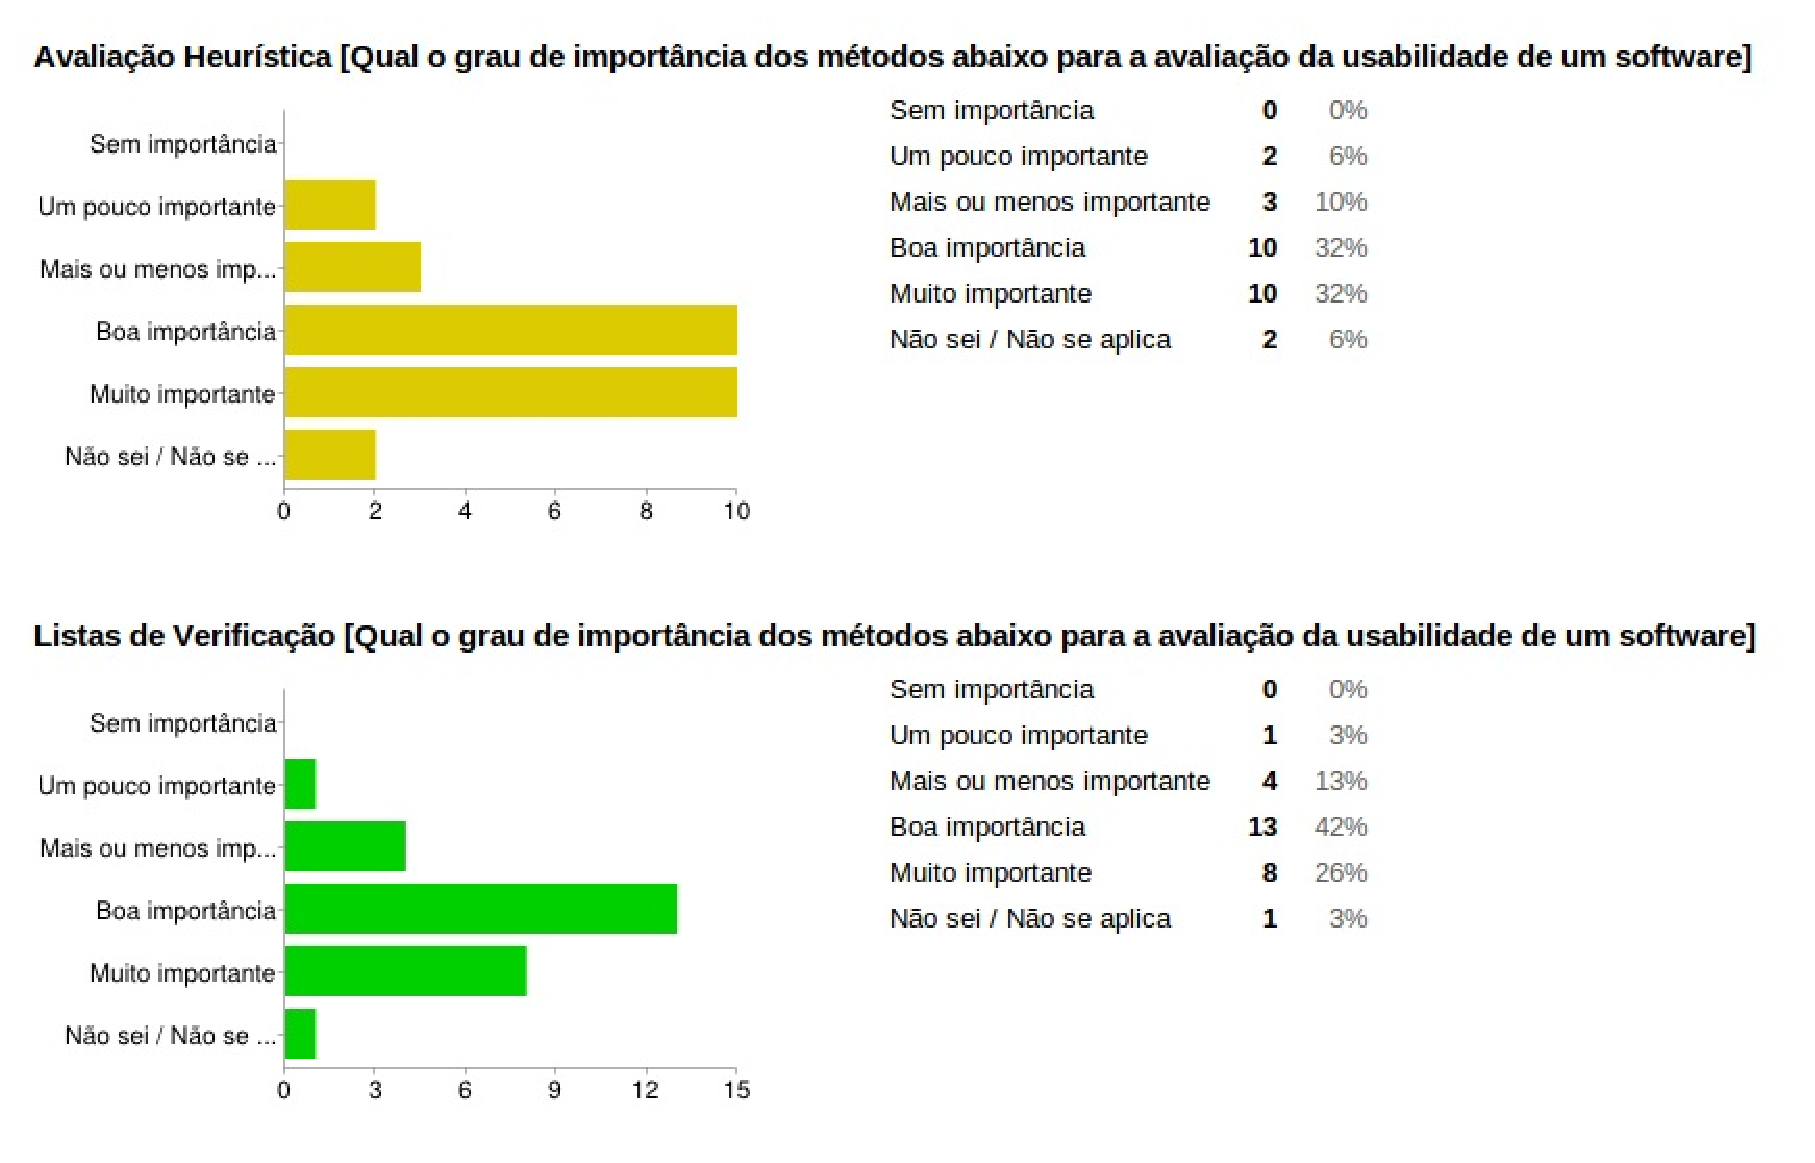
\includegraphics[keepaspectratio=true,scale=0.55]
      		{figuras/avalia1.eps}
    	\label{check04}
		\caption{Técnicas de avaliacao - Heurísticas e Listas de Verificação}
	\end{figure}
		
		Mais de 60\% informaram que as avaliações feitas por heurísticas e listas de verificação são de boa ou muita importância.
	
	\begin{figure}[!h]
    	\centering
    	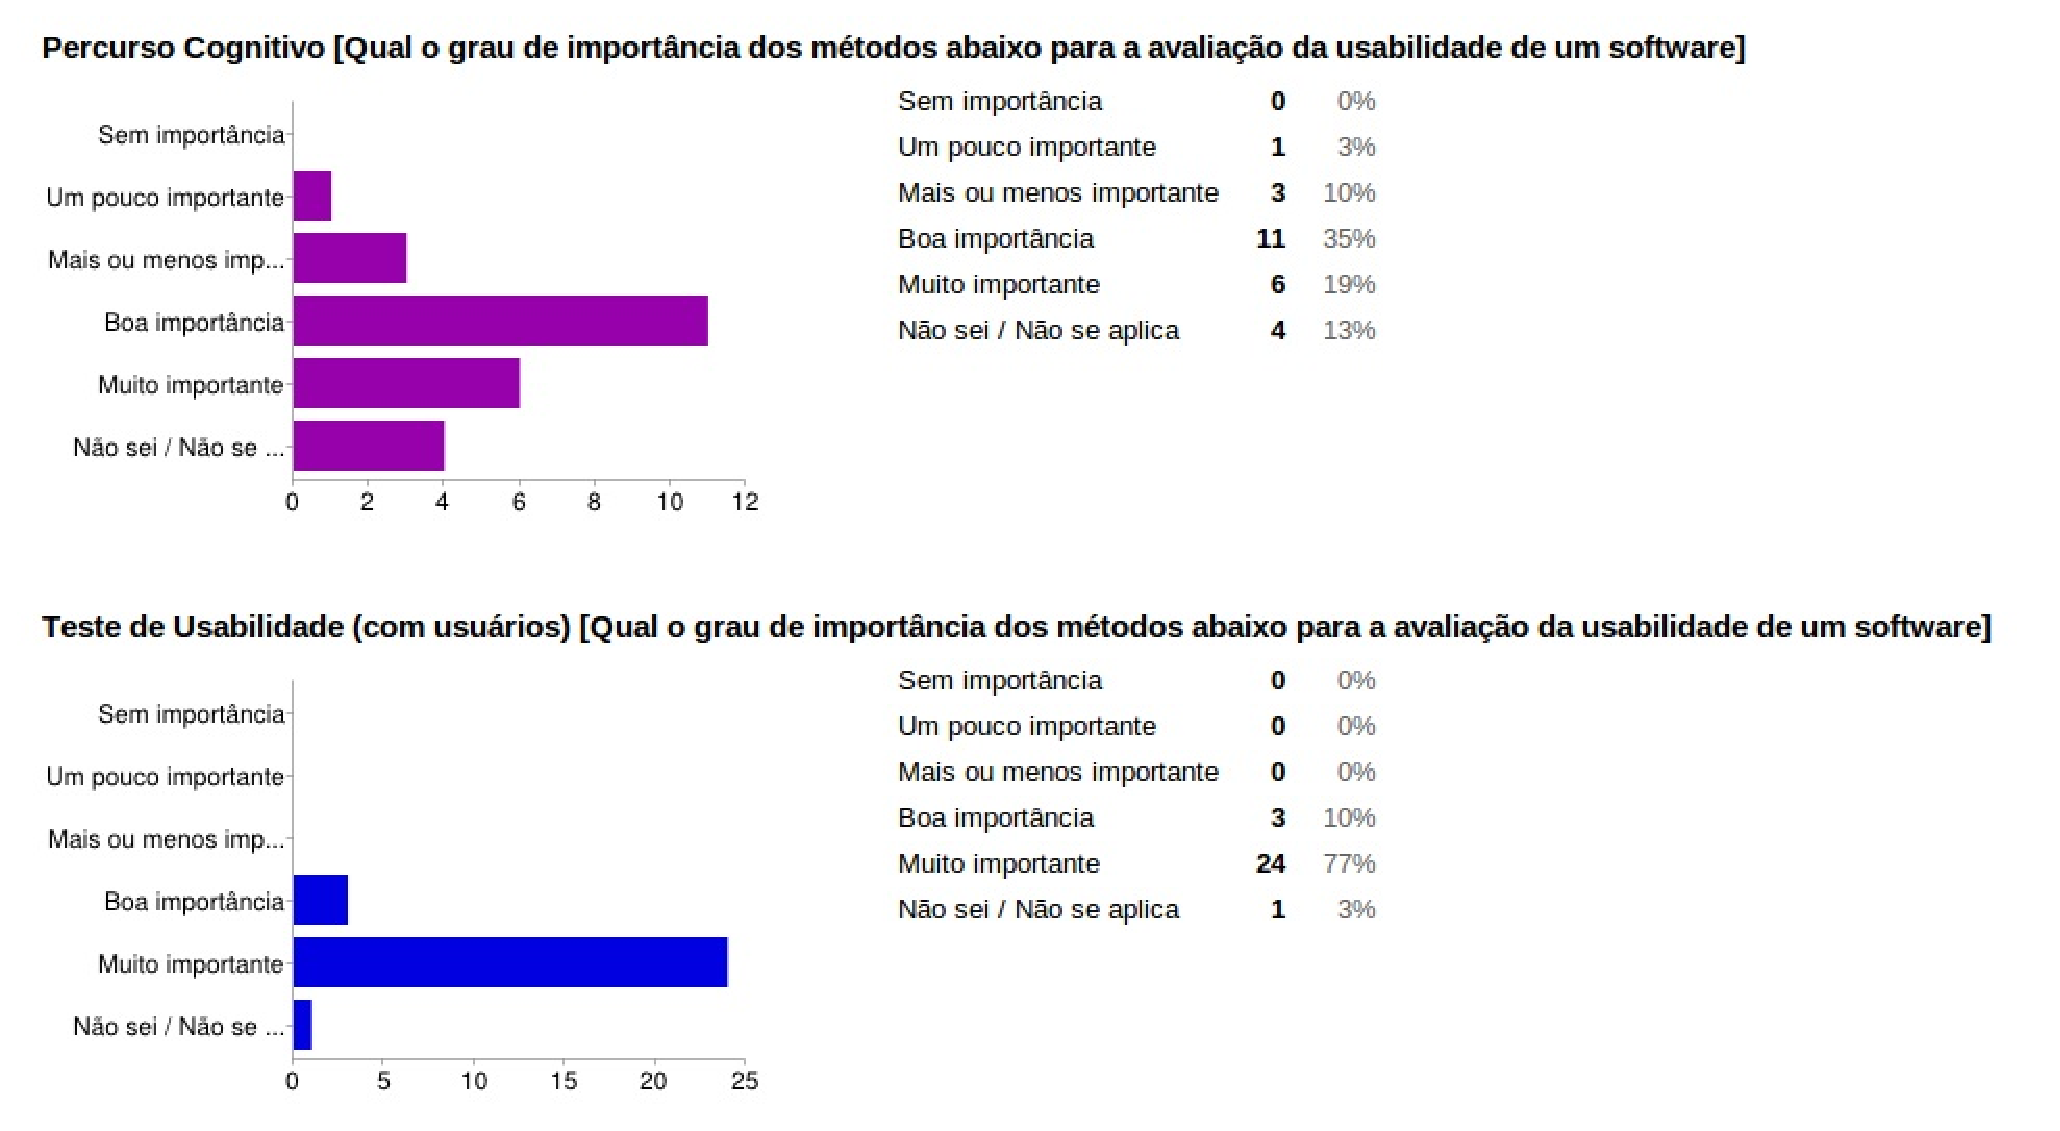
\includegraphics[keepaspectratio=true,scale=0.55]
      		{figuras/avalia2.eps}
    	\label{check04}
		\caption{Técnicas de avaliação - Percursos Cognitivos e Testes de Usabilidade}
	\end{figure}

		Os Testes de Usabilidade foram o que mais apresentaram importância para os pesquisados, sendo 77\% muito importante e 10\% boa importância.	